\documentclass[a4paper,11pt]{report}
\usepackage[utf8x]{inputenc}

\usepackage{lmodern}
\usepackage[T1]{fontenc}

\usepackage{amsmath}
\usepackage{amssymb}

\usepackage{graphicx}
% Title Page
\title{Calibration of scientific space-craft antennas}
\author{T.H. Oswald and H.O. Rucker}


\begin{document}
\maketitle

\begin{abstract}

\end{abstract}
\chapter{Introduction}
Antennas are electrical elements that can emit and receive electromagnetic radiation. An other way to describe the use of an antenna is to say that they are the interface between free wave propagation and guided wave propagation [Statement of Rucker 2003]\\

Two types of antennas can be found on most spacecraft. One type is the antenna required for communication between the spacecraft and the ground station or other spacecraft. This antenna is usually a form of dish antenna which is optimized for transmitting and receiving radiation of short wavelength in a well defined direction. This report is not about this type of antennas, though the principles could also be applied to them.\\ 

This report is about the other type of antennas, scientific antennas which are used to measure radiation created by physical processes driven by the dynamics of the universe. They are usually monopoles, dipoles or spherical probes, optimized for lower frequencies, from quasi-static to a frequency of a few tenth of Megahertz. They have a lower directivity, since radiation arrives from any direction. While spherical probes have advantages in dense plasma environment, they lack the necessary sensitivity when they are used to measure low frequency electromagnetic waves so monopoles and dipoles are more common. They can be made of wires or metal tubes. Wires can only be used on rotating spacecraft when centrifugal forces are used to keep them straight. Antennas made of wires can have a very low weight per unit length, so these antennas can be more than 100m long. Antennas made of metal tubes can be found on many non-rotating spacecraft. They can be between 1m and 15m long and are deployed when the spacecraft is in space. Different deploying mechanisms are in use. Most antennas of this kind are conically shaped, so the diameter at the root is larger than at the tip of the antenna.\\

Some antennas are mounted directly at the spacecraft hull, some are mounted on a boom which is made of insulating material. In the most preferable configuration 3 antennas are mounted in mutual orthogonal directions. This configuration is best for applying goniopolarimetry, i.e. the procedure of finding the direction of incidence of the received radiation and its state of polarization.\\

For a correct interpretation of the measured data, the reception behavior of the antennas must be known to a high degree of accuracy. This behavior, in turn is not easy to determine, because there are some factors which alter the antenna properties in a way which is hard to determine. Some of the most important factors are.

\begin{itemize}
 \item The shape of the spacecraft body.
\item The surrounding plasma.
\item The capacitances of the load of the antenna, i.e. the receiver, the mounting and the cable which is feeding the signal to the receiver.
\end{itemize}

To determine the influence of the mentioned influences is the procedure of calibration, the content of this report.\\

The larger part of calibration is about the first influence, the influence of the spacecraft body. To prevent potential differences between different parts of the spacecraft, the outer skin has to be made of conducting material. Since the measured entity is essentially the potential difference between the antenna monopole and the rest of the spacecraft (ground), the spacecraft body acts as an antenna itself. It can be seen as the second branch of a dipole. But since the spacecraft body does not have the shape of a monopole, the reception properties of the spacecraft body can not be determined by analytical means or by intuitive reasoning. Hence, more sophisticated methods must be used.\\

The influence of the surrounding plasma is a very complicated subject. When the plasma density is small, the influence is negligible and the antennas can be treated as if they where operating in free space. In certain regimes, however when a superposition of different plasma-waves are measured by the antenna, this approach is not feasible. Additionally the frequency also determines the need whether to consider plasma or not. In plasma there exist two types of waves, electromagnetic and electrostatic waves. By measuring only the electric field component, there is no way of telling weather the received wave belongs to one group or the other. To classify the waves, a magnetic measuring instrument, a magnetometer or magnetic (loop) antenna must be used in combination with the electric field measurement. Electrostatic waves do not have a magnetic field, so when the disturbance can also be seen on the magnetometer, it is an electromagnetic disturbance.\\

Electrostatic waves are heavily damped by a mechanism which is called Landau-Damping, so electrostatic waves are only expected to be found at the source region. And the frequency of electrostatic waves is directly connected to the density of the plasma in the source region. Most spacecraft operate in a regime where the electrostatic waves which are created by thermal effects, have a very low frequency, well below the frequency of the electromagnetic radiation of interest. Thus there is no ambiguity possible. By measuring the electrostatic waves, the plasma density and temperature can be estimated. This procedure is called Quasi-thermal Noise Spectroscopy (QTN).\\

Because of the reasons, mentioned above, it is not usual, that the magnetometer or magnetic antenna is used in combination with the electric antennas, and therefore they are not part of this report. It should be mentioned, that measuring the magnetic component of electromagnetic waves is extremely difficult, since the relation of electric to magnetic field-strength has a magnitude of c, the speed of light in vacuum. If it is measured despite of the sensitivity problems, the result is very valuable, though, since due to Maxwell's equation of solenoidity ($\nabla \cdot \mathbf{B}=0$) the wave-vector $\mathbf{k}$ has to be perpendicular to the plane of rotation of the magnetic field vector. For the electric field component this is only true in vacuum.\\

The base capacitances are the easiest of the influences to be considered. They can be computed analytically. The problem here is to determine the magnitude the capacitances. For an accurate calibration process they have to be measured on the actual equipment.

\chapter{The physics of the antennas}
\section{The effective length vector}
\subsection{Receiving antennas}

The antennas, this report is about, consist of one or two conducting metal rods or wires. When a fluctuation electric field is hits the antenna, a current is induced in each antenna branch. Due to the induced current, the feeding point at the antenna base has a certain potential. The potential difference, or voltage between the feeding points of the two dipole branches, or the monopole and ground (i.e. the spacecraft body in this application) is measured. \\

At the frequencies, space-based radio experiments work, the wavelength is much longer then the length of the antennas, so

\begin{equation}
 \lambda \gg l
\end{equation}

So we are talking about short antennas. When a quasi-static electric field hits a straight dipole antenna, the induced voltage between the open feed points is

\begin{equation}
 V_o=\frac{1}{2} \mathbf{E}\cdot \mathbf{l}
\end{equation}

where E is the incident electric field and $\mathbf{l}$ is the vector which represents the dipole. Other antenna shapes produce similar equations. For instance the open feed voltage of an antenna consisting of 2 spherical probes is

\begin{equation}
 V_o=\mathbf{E}\cdot \mathbf{l}
\end{equation}

where the length of l is the distance between the 2 probes. An effective length vector $\mathbf{l_{eff}}$ can be defined such that the open feed Voltage is

\begin{equation}
 V_o=\mathbf{E}\cdot \mathbf{l_{eff}}
\end{equation}

Defined this way, the effective length vector is a very important entity for describing the behavior of a receiving antenna. It can also be derived for a transmitting antenna which is not so easy to derive.

\subsection{Transmitting antennas}
\subsubsection{Generation of electromagnetic waves}
In general, electromagnetic waves are created as result of a change in the distribution of charges and currents, that is by the acceleration of charges. Radio waves, in particular, are created as result of oscillating electrons in the metallic structure of an antenna. To fully describe the process of the generation on EM waves, a quantumelectrodynamical treatment is necessary. Also by using only classical arguments, a phenomenological description can be given.\\

To describe the generation of electromagnetic waves, the use of potential fields is useful. These fields time dependent on space and time. The potential field at point $\mathbf{r}$ depends on the situation of the source at point $\mathbf{\acute{r}}$ at the time when the EM wave has left the source, that is at the time $\frac{|\mathbf{\acute{r}}-\mathbf{r}|}{c}$ before. \\

Two fields are needed, a scalar field, and a vector field. The rules are:

\begin{eqnarray}
\mathbf{B}&=&\nabla \times \mathbf{A} \label{rule_B}\\
\mathbf{E}&=&-\frac{\partial \mathbf{A}}{\partial t}-\nabla \phi \label{rule_E}
\end{eqnarray}

The potentials can be seen as the link between the physical fields and the currents and charges. The  fields, in turn, underlie the rules, given by Maxwell's equations, which are shown in appropriate form.

\begin{eqnarray}
\nabla \cdot \mathbf{E}&=&\frac{\rho}{\varepsilon_0}\label{maxwell1}\\
\nabla \cdot \mathbf{B}&=&0\label{maxwell2}\\
\nabla \times \mathbf{E}&=&-\frac{\partial \mathbf{B}}{\partial t}\label{maxwell3}\\
\frac{1}{\mu_0}\nabla \times \mathbf{B}&=&\mathbf{j}+\varepsilon_0 \frac{\partial \mathbf{E}}{\partial t}\label{maxwell4}
\end{eqnarray}

The potential fields are not unique, since one can add another vector field to \textbf{A} without changing the physics, as long as the rotation of the additional field is zero. In the same way, one can add a new scalar field to $\phi$, as long as its gradient is zero. Also, it is useful to apply another restriction to the fields, namely

\begin{equation}\label{lorenz}
\nabla \cdot \mathbf{A}=-\varepsilon_0 \mu_0\frac{\partial \mathbf{\phi}}{\partial t}
\end{equation}


This equation is called the Lorentz gauge. It has the effect bringing a symmetry into the equations and makes electrodynamics compatible with special relativity. Now we have all equations which are necessary to build wave equations for the potentials. First, one has to put equation (\ref{rule_B}) into Faraday's law:

\begin{equation}
\nabla \times \left( \mathbf{E}+\frac{\partial \mathbf{A}}{\partial t} \right) = 0
\end{equation}

So the whole term in the brackets can be expressed as gradient of a scalar potential, since the rotation of a gradient is always zero.

\begin{equation}\label{expressed_as_gradient}
\mathbf{E}+\frac{\partial \mathbf{A}}{\partial t} = -\nabla \phi
\end{equation}

Using equations (\ref{expressed_as_gradient})  and (\ref{rule_B}), one can write Ampere's law as

\begin{equation}
\nabla \times ( \nabla \times \mathbf{A} ) =\mu_0 \mathbf{j}-\mu_0 \varepsilon_0 \frac{\partial^2 \mathbf{A}}{\partial t^2}- \mu_0 \varepsilon_0 \nabla \left( \frac{\partial \mathbf{\phi}}{\partial t} \right)
\end{equation}


By using a well known identity of vector analysis for the rotation of the rotation of a vector field, one gets

\begin{equation}
\nabla^2 \mathbf{A} - \mu_0 \varepsilon_0 \frac{\partial^2 \mathbf{A}}{\partial t^2} =-\mu_0 \mathbf{j}+\nabla \left( \nabla \cdot \mathbf{A} + \mu_0 \varepsilon_0 \frac{\partial \mathbf{\phi}}{\partial t} \right)
\end{equation}


and by using the Lorentz gauge, one gets the inhomogeneous vector Helmholtz equation.

\begin{equation}
\nabla^2 \mathbf{A} - \mu_0 \varepsilon_0 \frac{\partial^2 \mathbf{A}}{\partial t^2} =-\mu_0 \mathbf{j}
\end{equation}



In the same way (\ref{expressed_as_gradient}) can be combined with Gauss's law with subsequent use of Lorentz gauge to yield the inhomogeneous scalar Helmholtz equation.

\begin{equation}
\nabla^2 \phi - \mu_0 \varepsilon_0 \frac{\partial^2 \phi }{\partial t^2} =-\frac{\rho }{\varepsilon_0 }
\end{equation}

In case of time harmonic sources, a Fourier transform in time can be applied and results in :

\begin{eqnarray}
\nabla^2 \mathbf{A} + \mu_0 \varepsilon_0 \omega^2 \mathbf{A}&=& -\mu_0 \mathbf{j} \label{HH1}\\
\nabla^2 \phi + \mu_0 \varepsilon_0 \omega^2 \phi  &=&-\frac{\rho }{\varepsilon_0 } \label{HH2}
\end{eqnarray}

The solution for the time-harmonic case is

\begin{eqnarray}
\phi (\mathbf{r},t) &=& \int_{V'} \frac{\rho ( \mathbf{r}' )}{4 \pi \varepsilon_0 |\mathbf{r} - \mathbf{r}'| } e^{-ik|\mathbf{r} - \mathbf{r}'| } dV' \label{dynamicharmonicsolution1}\\
 \mathbf{A}(\mathbf{r},t) &=& \int_{V'} \frac{\mu_0 \mathbf{j} ( \mathbf{r}' )}{4 \pi  |\mathbf{r} - \mathbf{r}'| \label{dynamicharmonicsolution2}} e^{-ik|\mathbf{r} - \mathbf{r}'| } dV'
 \end{eqnarray}


The general form that does not rely on a time harmonic source, is

\begin{eqnarray}
\phi (\mathbf{r},t) &=& \int_{V'} \frac{\rho ( \mathbf{r}', t-|\mathbf{r} - \mathbf{r}'| /c  )}{4 \pi \varepsilon_0 |\mathbf{r} - \mathbf{r}'| } dV' \label{dynamicsolution1}\\
 \mathbf{A}(\mathbf{r},t) &=& \int_{V'} \frac{\mu_0 \mathbf{j} ( \mathbf{r}', t-|\mathbf{r} - \mathbf{r}'| /c  )}{4 \pi  |\mathbf{r} - \mathbf{r}'| \label{dynamicsolution2}}  dV'
 \end{eqnarray}

\subsubsection{The Hertz'ian Dipole}
A Hertz'ian Dipole is the simplest hypothetical construct that is able to emit electromagnetic radiation. It is not realizable in reality, due to two facts. First, it is supposed to be infinitesimal short, and the current along the dipole is taken to be constant. The Hertz'ian Dipole would represent a quantum mechanical process, where an electron changes its position and decreasing its potential energy by this change under emission of a photon. Following facts are true for the Hertz'ian Dipole.


\begin{eqnarray}
\frac{l}{z} &\geq& z' \label{hd1} \\
l &\ll& \lambda \label{hd2} \\
l &\rightarrow& 0 \label{hd3} \\
I=\frac{dq}{dt} &=& \omega q_0 \cos{\omega t} = I_0 \cos{\omega t} \label{hd4} \\
P=ql &=& P_0 \sin{\omega t}  \label{hd5} \\
P_0=ql_0 &=& q_0 l \label{hd6}
\end{eqnarray}

$P$ is the dipole moment. Equation (\ref{hd1}) means that only locations which are far away from the dipole, in relation to its size are taken into account. Equations (\ref{hd2}) and (\ref{hd3}) mean that the dipole is short in relation to the wavelength and it is infinitesimal small, in general. Equation (\ref{hd4}) says that the current which produces the radiation is oscillating harmonically, has the same phase along the dipole, and the same amplitude (which is physically impossible for a real antenna). Finally, equations (\ref{hd5}) and (\ref{hd6}) describe the dipole moment.\\


Due to the assumptions and the symmetry, one can use the following simplifications:

\begin{eqnarray}
  \mathbf{j} &=& I_z\mathbf{ \hat{z}'} \delta (x') \delta (y') \label{hd_simpli_1}\\
\mathbf{A} &=& A_z \label{hd_simpli_2} \\
|\mathbf{r}-l_z\mathbf{ \hat{z}'}| &\approx& r \label{hd_simpli_3}\\
t-|\mathbf{r}-l_z\mathbf{ \hat{z}'}| / c &\approx& t-\frac{r}{c}\label{hd_simpli_4}
\end{eqnarray}

\begin{equation}\label{simple_potential_solution}
 A_z (\mathbf{r},t) = \frac{ \mu_0}{4 \pi}\int^{\frac{l}{2}}_{-\frac{l}{2}} \frac{ I ( z', t- r/c  )}{r}  dV'
\end{equation}

Under the presumption that the current $I_z$ is constant along the dipole, on can substitute the integral with the multiplication by the length of the dipole.

\begin{equation}\label{simple_potential_solution2}
 A_z (\mathbf{r},t) = \frac{ \mu_0 I ( z', t- r/c  ) l}{4 \pi r}
\end{equation}

When the source has a is time harmonic behavior:

\begin{equation}\label{simple_potential_solution_timeharmonic}
 A_z (\mathbf{r},t) = \frac{\mu_0 I l}{4 \pi r} e^{-ikr }
\end{equation}


Now one can use the Lorentz gauge (\ref{lorenz}) to derive the scalar potential. Of course, the Lorentz gauge can be simplified, first. One gets:

\begin{eqnarray}
\frac{\partial A_z }{\partial z}&=&-\varepsilon_0 \mu_0\frac{\partial \mathbf{\phi}}{\partial t} \label{lorenz_simplified} \\
\Rightarrow \frac{\partial }{\partial z} \left(  \frac{ \mu_0 I l}{4 \pi r} e^{-ikr } \right) &=&-\varepsilon_0 \mu_0\frac{\partial \mathbf{\phi}}{\partial t} \nonumber \\
\Rightarrow \frac{\partial \mathbf{\phi}}{\partial t} &=&-  \frac{\partial }{\partial z} \left(  \frac{ I l}{4 \pi r \varepsilon_0} e^{-ikr } \right)  \nonumber\\
&=&  \frac{ I l}{4 \pi \varepsilon_0} e^{-ikr } 2z \left( \frac{1}{r^2} + \frac{1}{r^3} \right) \label{diff_eq_scalar_pot}
\end{eqnarray}


The last step of this derivation can be achieved by using the product rule and the chain rule, since $r=\sqrt{x^2+y^2+z^2}$. For the time harmonic case, one can use a Fourier transform in time: $\phi (\mathbf{r},t) \rightarrow \phi (\mathbf{r},\omega)$ and $\frac{\partial }{\partial t} \rightarrow i \omega$.

\begin{eqnarray}
\frac{\partial \phi}{\partial t} &=& i \omega \phi\\
&=& \frac{ I l}{4 \pi \varepsilon_0} e^{-ikr } 2z \left( \frac{1}{r^2} + \frac{1}{r^3} \right)  \nonumber \\
\Rightarrow \phi &=& \frac{ I l z}{2 \pi \varepsilon_0 i \omega} e^{-ikr } \left( \frac{1}{r^2} + \frac{1}{r^3} \right) \label{solution_scalar_pot_hd}
\end{eqnarray}

When only the far field is considered, there is no harm done, by neglecting the $\frac{1}{r^3}$ term, because it falls off very rapidly. So

\begin{equation}\label{solution_scalar_pot_hd_ff}
\phi = \frac{ I l z}{2 \pi \varepsilon_0 i \omega r^2} e^{-ikr }
\end{equation}

The next step is to calculate the fields by using (\ref{rule_B}) and (\ref{rule_E}). For this purpose, it is useful to switch to a spherical reference frame, where $\mathbf{\hat{z}}=\mathbf{\hat{r}} \cos \theta - \mathbf{\hat{\theta}} \sin \theta$. From equation (\ref{simple_potential_solution_timeharmonic}) one gets

\begin{equation}\label{simple_potential_solution_timeharmonic_sherical_ref}
 \mathbf{A}_z (\mathbf{r},t) = (\mathbf{\hat{r}} \cos \theta - \mathbf{\hat{\theta}} \sin \theta) \frac{\mu_0 I l}{4 \pi r} e^{-ikr }
\end{equation}


So

\begin{eqnarray} \label{get_B_hd}
\mathbf{B}&=&\nabla \times \mathbf{A} \\
&=&\frac{1}{r^2 \sin \theta}\left|%
\begin{array}{ccc}
 \mathbf{ \hat{r}} & r\mathbf{\hat{\theta}} & r \sin \theta \mathbf{\hat{\phi}} \\
  \frac{\partial }{\partial r} & \frac{\partial }{\partial \theta } & \frac{\partial }{\partial \phi } \\
  A_r & rA_{\theta } & r \sin \theta A_{\phi} \\
\end{array}%
\right|\\
&=&\mathbf{ \hat{\phi}} \frac{1}{r} \left[ \frac{\partial }{\partial r} \left( rA_\theta \right) - \frac{\partial }{\partial \theta } (A_r)\right] \nonumber \\
&=& \mathbf{\hat{\phi}}\frac{\mu_0 I l}{4 \pi r} \left[ -\sin \theta \frac{\partial }{\partial r} \left(   e^{-ikr } \right) - \frac{e^{-ikr }}{r} \frac{\partial }{\partial \theta } (\cos \theta )\right] \nonumber \\
&=& \mathbf{\hat{\phi}} \frac{i \mu_0 k I l}{4 \pi r} e^{-ikr } \left[ 1+ \frac{1}{kir}\right] \sin \theta \nonumber
\end{eqnarray}

and

\begin{eqnarray} \label{get_E_hd}
\mathbf{E}&=& \frac{1}{i\omega \varepsilon_0 \mu_0} \nabla \times \mathbf{B} \\
&=&\frac{i}{ \omega \mu_0 \varepsilon_0} \nabla \times\mathbf{ \hat{\phi}} \left( \frac{i \mu_0 k I l}{4 \pi r} e^{-ikr } \left[ 1+ \frac{1}{kir}\right] \sin \theta \right) \\
&=&\frac{  I l}{4 \pi \varepsilon_0 c} \nabla \times \mathbf{\hat{\phi}} \left( e^{-ikr } \left[  \frac{ 1}{ r}+ \frac{1}{kir^2}\right] \sin \theta \right)
\end{eqnarray}

Performing the curl of the term:

\begin{eqnarray}
&&\nabla \times \left( e^{-ikr } \left[  \frac{ 1}{ r}+ \frac{1}{kir^2}\right] \sin \theta \right)\nonumber \\
&&=\mathbf{\hat{r} }\left[ \frac{1}{r \sin \theta} \frac{\partial }{\partial \theta } \left( \sin \theta \left( e^{-ikr } \left[  \frac{ 1}{ r} +\frac{1}{kir^2}\right] \sin \theta \right) \right) \right] \nonumber \\
&&-\mathbf{ \hat{\theta}} \left[ \frac{1}{r} \frac{\partial }{\partial r } \left( r \left( e^{-ikr } \left[  \frac{ 1}{ r}+ \frac{1}{kir^2}\right] \sin \theta \right) \right) \right]\nonumber \\
&&=\mathbf{\hat{r}} \left[ \frac{1}{ \sin \theta} e^{-ikr } \left[  \frac{ 1}{ r^2} +\frac{1}{kir^3}\right] \frac{\partial }{\partial \theta } \left( \sin^2 \theta     \right) \right] \nonumber \\
&&-\mathbf{ \hat{\theta}} \left[ \frac{\sin \theta}{r} \frac{\partial }{\partial r } \left(   e^{-ikr } \left[  1 + \frac{1}{kir}\right]  \right) \right]\nonumber\\
&&=\mathbf{\hat{r}} \left[ \frac{1}{ \sin \theta} e^{-ikr } \left[  \frac{ 1}{ r^2} +\frac{1}{kir^3}\right]  2 \sin \theta \cos \theta     \right] \nonumber \\
&&- \mathbf{\hat{\theta}} \left[ \frac{\sin \theta}{r}  e^{-ikr } \left(  -ik   \left[  1 + \frac{1}{kir}\right]+   \left[ - \frac{1}{kir^2}\right] \right) \right] \nonumber \\
&&=\mathbf{\hat{r} }\left[ e^{-ikr } \left[  \frac{ 1}{ r^2} +\frac{1}{kir^3}\right]   2  \cos (\theta )   \right] \nonumber \\
&&+\mathbf{ \hat{\theta}} \left[ \frac{ik \sin \theta}{r}  e^{-ikr } \left( 1 + \frac{1}{kir}+  \frac{1}{(kir)^2} \right) \right]
\end{eqnarray}

Hence

\begin{eqnarray} \label{get_E_hd}
&&\mathbf{E}=\\
&&=\frac{  I l}{4 \pi \varepsilon_0 c} \left\{ \mathbf{\hat{r}} \left[ e^{-ikr } \left[  \frac{ 1}{ r^2} +\frac{1}{kir^3}\right]   2  \cos (\theta )   \right] \right. \nonumber\\
&&\left. +\mathbf{ \hat{\theta}} \left[ \frac{ik \sin \theta}{r}  e^{-ikr } \left( 1 + \frac{1}{kir}+  \frac{1}{(kir)^2} \right) \right] \right\} \nonumber  \\
&&=\sqrt{\frac{\mu_0}{ \varepsilon_0}}\frac{  I l}{4 \pi r} e^{-ikr } \left\{ \mathbf{\hat{r}} \left[  \left[  \frac{ 1}{ r} +\frac{1}{kir^2}\right]   2  \cos (\theta )   \right]  \right. \nonumber\\
&&\left.+\mathbf{ \hat{\theta}} \left[ ik \sin \theta   \left( 1 + \frac{1}{kir}+  \frac{1}{(kir)^2} \right) \right] \right\} \nonumber  \\
&&=\frac{i k \eta_0 I l}{4 \pi r} e^{-ikr } \left\{ \mathbf{\hat{r} }\left[  \left[  \frac{ 1}{ i k r} +\frac{1}{(kir)^2}\right]   2  \cos (\theta )   \right] \right. \nonumber\\
&&\left.+\mathbf{ \hat{\theta}} \left[  \sin \theta   \left( 1 + \frac{1}{kir}+  \frac{1}{(kir)^2} \right) \right] \right\} \nonumber
\end{eqnarray}


In the far field zone, which means at a distance of more than a few antenna lengths, $kr \gg 1$, so these terms  that dominated the near field zone, can now be neglected. One can use simplified versions of the equations, when describing the far field.

\begin{eqnarray}
\mathbf{B} &=& \mathbf{\hat{\phi}} \frac{i \mu_0 k I l}{4 \pi r} e^{-ikr } \sin \theta \label{fraunhofer_B} \\
\mathbf{E} &=&\mathbf{ \hat{\theta}} \eta_0 \frac{i k I l}{4 \pi r} e^{-ikr } \sin \theta \label{fraunhofer_E} 
\end{eqnarray}


These simplifications, are called \emph{Fraunhofer Farfield Approximation}, indicated in the equations by the index \emph{ff}. Those equations were derived by using the example of a Hertz'ian Dipole, but the principle is generally true. A simplified integral equation can be derived for the vector potential, that is particularly useful. Starting at equation (\ref{dynamicharmonicsolution2}), one gets

\begin{equation}\label{fraunhofer_A}
 \mathbf{A}_{ff}(\mathbf{r},t) = \frac{\mu_0}{4 \pi r} e^{-ikr} \int_{V'} \mathbf{j}(\mathbf{r}') e^{ik \mathbf{\hat{r}} \cdot \mathbf{r}' } dV'
\end{equation}


Using this solution, one can produce a simplified formula for calculating the electric and magnetic far-field approximations for time harmonic sources by performing a Fourier transform in time and space.

\begin{eqnarray}
\mathbf{H}_{ff} (\mathbf{k},\omega)&=& \mathfrak{FT} \left\{ \frac{1}{\mu_0} \nabla \times \mathbf{A}_{ff}(\mathbf{r},t) \right\} = - \frac{1}{\mu_0} ik\mathbf{\hat{r}} \times \mathbf{A}_{ff}(\mathbf{k},\omega) \label{rule_Hff}\\
\mathbf{E}_{ff} (\mathbf{k},\omega)&=&  \mathfrak{FT} \left\{ \frac{1}{i\omega \varepsilon_0 } \nabla \times \mathbf{H}_{ff}(\mathbf{r},t) \right\}= -\eta_0 \mathbf{\hat{r}} \times \mathbf{H}_{ff}(\mathbf{k},\omega) \\
&=& i \omega \mathbf{\hat{r}} \times ( \mathbf{\hat{r}} \times \mathbf{A}_{ff}(\mathbf{k},\omega)) \label{rule_Eff}
\end{eqnarray}

\subsubsection{Real antennas and their properties}
The simplest, real antenna is the short dipole as described in the last section. A short dipole has a length that is small in relation to the wavelength, but not infinitesimal. The current distribution along the antenna is not constant along the antenna, but

\begin{equation}\label{shd_current}
 \mathbf{j} = \mathbf{\hat{z}} I(z') \delta (x') \delta (y')
\end{equation}

Since the dipole is short in relation to the wavelength, the phase is the same at any point of the antenna. This simplifies the situation to some extent. Putting (\ref{shd_current}) in (\ref{fraunhofer_A}), one gets the vector potential:


\begin{equation}\label{shd_A}
 \mathbf{A}_{ff}(\mathbf{r},t) = \mathbf{\hat{z} }\frac{\mu_0}{4 \pi r} e^{-ikr} \int_{-\frac{l}{2}}^{\frac{l}{2}} I(z') e^{ik z'\cos \theta } dz'
\end{equation}

Due to the constant phase, this simplifies to

\begin{equation}\label{shd_A_simpl}
\mathbf{A}_{ff}(\mathbf{r},t) = \mathbf{\hat{z}} \frac{\mu_0}{4 \pi r} e^{-ikr} \int_{-\frac{l}{2}}^{\frac{l}{2}} I(z') dz'
\end{equation}

At this point it is possible to define the effective antenna length $l_{eff}$ in a way that

\begin{equation}\label{defin_leff}
Il_{eff}= \int_{-\frac{l}{2}}^{\frac{l}{2}} I(z') dz'
\end{equation}

Then

\begin{equation}\label{shd_A_solution}
\mathbf{A}_{ff}(\mathbf{r},t) = \mathbf{\hat{z}} \frac{\mu_0 I l_{eff}}{4 \pi r} e^{-ikr}
\end{equation}

If the current was constant along the wire, like in the Hertz'ian Dipole, the effective length would have the same magnitude than the physical length, which is not possible in reality. It is difficult to determine the actual current distribution, the only thing that can be said for sure is, that the current must be zero at all times at the tips of the antenna. For many purposes, including a short dipole, a linear current distribution, which is the easiest to deal with, is a good estimation. In this case, according to equation (\ref{defin_leff}), one can calculate the effective length.

%\begin{figure}
%  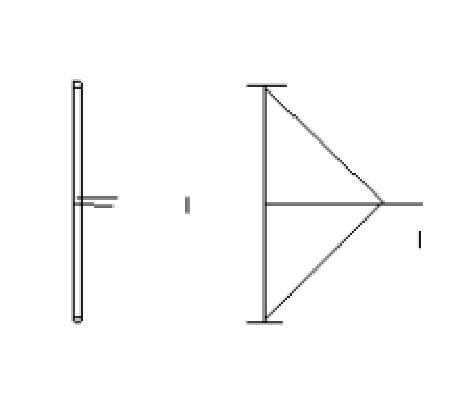
\includegraphics[width=12cm]{curr_distr_shd}\\
%  \caption{Linear current distribution}\label{fig_curr_distr_shd}
%\end{figure}

\begin{eqnarray}
I&=&I_0 \left( \frac{\frac{l}{2}-|z'|}{\frac{l}{2}}\right) \label{l_eff_shd_1} \\
\Rightarrow  l_{eff}&=& \frac{1}{I} \int_{-\frac{l}{2}}^{\frac{l}{2}} I_0 \left( \frac{\frac{l}{2}-|z'|}{\frac{l}{2}}\right) dz' \label{l_eff_shd_2} \\
&=&\frac{l}{2} \nonumber
\end{eqnarray}

This is the same result as for the receiving antenna. The physical fields can be calculated in the same way as for the Hertz'ian Dipole, one has just to use the effective dipole length instead of the geometric length.\\

It should be emphasized that the effective length is defined using the far-field approximation, so it is an entity related to the far-field. When calculating the effective length vector, only the far-field must be used and not the full field solution, even if it is known.\\

\subsection{Practical computation}
When the computation of the effective length vectors is required, there are generally two different methods. Both are using the model of a transmitting antenna. Due to the reciprocity theorem, the results are applicable also to receiving antennas.\\

When the current distribution is known, one can use the following volume integral.

\begin{equation}\label{eq:heff}
\textbf{l}_{eff}=\frac{1}{I}\int \mathbf{j}(\mathbf{r}')e^{\imath \mathbf{k} \cdot \mathbf{r}'} dV'
 \end{equation}

The other method uses the Potential field. See eq. \ref{shd_A_solution}.

\begin{equation}\label{l_eff_with_1}
 \mathbf{l}_{eff}(\mathbf{r}) =\frac{4 \pi r}{\mu_0 I }\mathbf{A}_{ff}(\mathbf{r},t) e^{i(\mathbf{k}\cdot \mathbf{r})}
\end{equation}

In reality, the 2 equations are equivalent. So the effective length vector is a function of direction. Since $A=A(\frac{1}{r}$, and the potential field is multiplied by $r$, the effective length vector does not depend on the distance, which is how it should be. For short antennas the effective lengths vectors should roughly be the same for all directions, so an appropriate method is to take the average over all computed directions. When the wavelength approaches the dimension of the antenna, this is not the case. In that case the effective length vector can be different for each different direction and averaging makes no sense in a physical way.\\

\subsection{The conversion of measured voltages to electric fields}
To convert measured voltages to electric fields in the spacecraft coordinate frame, one can use the formula \cite{bale08}:

\begin{equation}
 \mathbf{E}=\mathbf{M}\cdot \mathbf{V}
\end{equation}
where

\begin{equation}\label{eq:conversion}
 \mathbf{M}=\left(
\begin{array}{ccc}
h_{eff,1} cos \theta_1 & h_{eff,1} sin \theta_1 sin \phi_1 & -h_{eff,1} sin \theta_1 cos \phi_1 \\
h_{eff,2} cos \theta_2  & h_{eff,2} sin \theta_2 sin \phi_2 & -h_{eff,2} sin \theta_2 cos \phi_2\\
h_{eff,3} cos \theta_3 & h_{eff,3} sin \theta_3 sin \phi_3 & -h_{eff,3}  sin \theta_3 cos \phi_3\\
\end{array}%
\right)^{-1}
\end{equation}

\section{Open and loaded antennas}
The voltage between the antenna and ground or between the two branches of the dipole is measured. The signal is amplified by using a pre-amplifier and then fed to the receiver. What happens then depends on the kind of experiment, the required product and the state of technology at the time of design of the hardware.\\

Regarding the data which should be sent to Earth, there are 3 common possibilities. 

\begin{itemize}
 \item The correlation parameters between the antennas
\item Frequency intensity data
\item The full waveform
\end{itemize}

At a ground based station, the full waveform is the best option, but since there is a limit to the amount of data which can be sent from a spacecraft to Earth, this is not an option. One solution to this problem is to send only data from short time spans which are triggered by certain events, the other solution is to make some signal processing on board and send only the advanced data product (i.e. the frequency intensity data) to Earth. Extracting only the correlation parameters from the signal can be done by an analogue signal processor and was common at the early space-missions. Advanced signal processing needs a digital signal processor on board, together with storage capabilities. The hardware requirements and therefore the space and mass of the required hardware is higher, but the data output of the experiment is much more sophisticated and useful.\\

Figure \ref{fig:equivalent_open} shows the equivalent circuit of a receiving antenna with open feeds. The antenna is represented by the antenna impedance $Z_a$. $Z_a$ is complex. The real part is called antenna resistance and is a measure for the sensitivity of the receiving antenna. The reactance is the imaginary part. At a short antenna, the reactance is negative, so the antenna acts like a capacitator. With shorter wavelength it becomes larger and at the so called half-wave-resonance it becomes inductive. The resistive term is usually small and can be neglected in the equivalent circuit. The antenna impedance depends on the frequency and is an important entity which should be computed during the process of calibration. The resistive term can be approximated as

\begin{equation}
 R_a=80\left(\frac{\pi f l}{c}\right)^2
\end{equation}
 
and the reactive term as

\begin{equation}
 C_a=\frac{\epsilon \pi l}{ln(\frac{2l}{d})-1}
\end{equation}

\cite{king56}, where $l$ is the effective lengths of the monopole or half dipole, $d$ is the diameter, $f$ is the frequency and $c$ is the speed of light in vacuum. It is common to construct a graph which plots antenna resistance and reactance as a function of frequency. Figure \ref{fig:impedance_plot} shows an example of such a graph. An other possibility is to plot the resistance against reactance.

\begin{figure}
  \noindent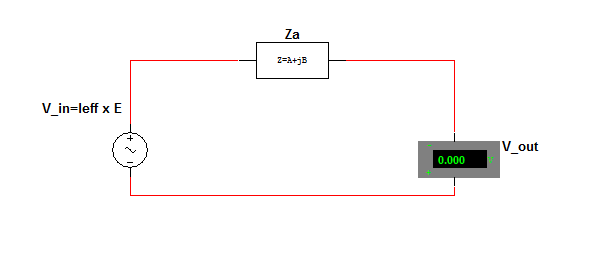
\includegraphics[width=12cm]{Ersatzschaltung_openfeed}
\caption{Equivalent circuit of an antenna with open feeds}
\label{fig:equivalent_open}
\end{figure}

\begin{figure}
  \noindent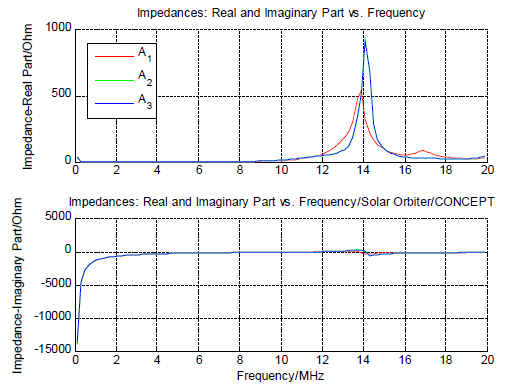
\includegraphics[width=12cm]{impedances_ex}
\caption{Example of an impedance plot}
\label{fig:impedance_plot}
\end{figure}

In reality the feeds are not open but loaded. In the receiver and the cable power is dissipated and they act as stray capacitances parallel to the antenna. Figure \ref{fig:equivalent_loaded} shows the equivalent circuit. The resistive part of the receiver is usually very high and can therefore be neglected at HF frequencies, so the load impedances can be modeled as load capacitances $C_l$. The range of the load capacitances can be $30-50pF$ for monopoles and $15-75pF$ for dipoles \cite{manning00}. It is desirable to keep the load capacitances as low as possible so also from this standpoint a dipole is preferable. The net effect of the load capacitances is to reduce the Voltage:

\begin{equation}
 V_l=V_o\frac{C_a}{C_a+C_l}
\end{equation}

The magnitudes of the effective length vectors are reduced by the same factor.

\begin{figure}
  \noindent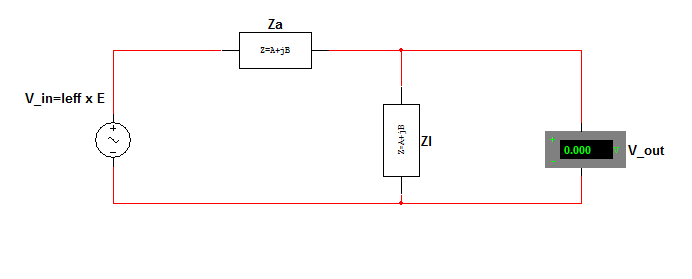
\includegraphics[width=12cm]{Ersatzschaltung_loadedfeed}
\caption{Equivalent circuit of a loaded antenna}
\label{fig:equivalent_loaded}
\end{figure}


\section{Other parameters to describe antenna behavior}
The effective length vectors and antenna capacitances turned out to be the most important parameters to describe the behavior of scientific space-borne antennas. There are, however other parameters which have a high content of useful information.

\subsection{The power pattern}
Above the quasi-static range, the effective length vectors depend on the direction of incidence of the received radiation and they have a significant imaginary part. Therefore they are not suitable to describe the antenna behavior of high frequencies. The concept of the power pattern is more useful in this case. The power pattern is a concept of the transmitting antenna, but due to the reciprocity principle, it can also be used for receiving antennas, as long as the plasma can be neglected.\\

The power pattern is the 2 dimensional surface which represents the energy flow radial outward from the electric center of the antenna, as a function of the direction, i.e. the angles $\theta$ and $\phi$.

\begin{equation}
 P(\theta,\phi)=|\mathbf{S}(\theta,\phi)|
\end{equation}

where $\mathbf{S}$ is the average Poynting vector which represents direction and magnitude of the average energy flow per unit area.

\begin{equation}
 \mathbf{S}(\theta,\phi)=\frac{E(\theta,\phi)^2}{\eta_0}[Wm^{-2}]
\end{equation}
 
where E is the magnitude of the amplitude of the electric field of the electromagnetic wave which propagates in direction $(\theta,\phi)$ (the electric field is NOT pointing in this direction). $\eta_0$ is the impedance of free space.\\

Often the normalized power pattern is used.

\begin{equation}
 P_n(\theta,\phi)=\frac{|\mathbf{S}(\theta,\phi)|}{|\mathbf{S}(\theta,\phi)|_{max}}
\end{equation}

$P_n$ is dimensionless and can be given in Decibel. Patterns can also be constructed with different fields, like electric field pattern or magnetic field pattern. Even components of fields can be used, for instance the horizontal component of the electric field. The pattern can be used to visualize the sensitivity of the antenna in a given direction.

\subsection{Gain and Directivity}
The directivity is the fraction of the maximum power to the average power. The average power is the transmitted power per area if the total power transmitted would be equally distributed in all direction, i.e. the antenna would be an isotropic radiator, which physically not possible.

\begin{equation}
 D=\frac{P(\theta,\phi)_{max}}{\frac{1}{4 \pi}\iint_{4\pi}P(\theta,\phi)d\Omega}
\end{equation}

The gain is the directivity reduced by an efficiency factor which reflects the losses at a real antenna in comparison to an ideal.

\begin{equation}
 G=kD
\end{equation}

k is always smaller than 1.

\section{The reciprocity principle}
In a simple sentence, the reciprocity states, that one can exchange the source of an electromagnetic wave, with the receiving antenna without changing the result, as long as the medium is linear and isotropic. It does not have to be homogeneous. This result is extremely important for antenna calibration, because it implies on can either use transmitting antennas (MoM) or receiving antennas (inflight calibration) to produce the same results. The reciprocity principle is not valid in magnetized plasma.

Defining two sets of sources, $[J_1 M_1, J_2 M_2]$, the field equation for time harmonic waves area

\begin{eqnarray}
 \nabla \times \mathbf{H_1} &=&  \mathbf{E_1}+ \mathbf{J_1}\\ \label{eq:rezifield1}
\nabla \times \mathbf{-E_1} &=&  \mathbf{H_1}+ \mathbf{M_1}\\
\nabla \times \mathbf{H_2} &=&  \mathbf{E_2}+ \mathbf{J_2}\\
\nabla \times \mathbf{-E_2} &=&  \mathbf{H_2}+ \mathbf{M_2} \label{eq:rezifield2}
\end{eqnarray}

By taking the in-product of \ref{eq:rezifield1} with $\mathbf{E_2}$ and the in-product of \ref{eq:rezifield2} with $\mathbf{H_1}$ and add the resulting equations, one gets

\begin{equation}
 - \nabla \cdot (\mathbf{E_1} \times \mathbf{H_2}- \mathbf{E_2} \times \mathbf{H_1})=\mathbf{E_1} \cdot \mathbf{J_2}+\mathbf{H_2} \cdot \mathbf{M_1} - \mathbf{E_2} \cdot \mathbf{J_1}-\mathbf{H_1} \cdot \mathbf{M_2}
\end{equation}

This is the Lorentz Reciprocity Theorem in its differential form. There exists also an integral form. By integrating both sides over the total volume and applying the divergence theorem on the left side, one gets

\begin{equation}
 - \iint_S (\mathbf{E_1} \times \mathbf{H_2}- \mathbf{E_2} \times \mathbf{H_1}) \cdot ds'=\iiint (\mathbf{E_1} \cdot \mathbf{J_2}+\mathbf{H_2} \cdot \mathbf{M_1} - \mathbf{E_2} \cdot \mathbf{J_1}-\mathbf{H_1} \cdot \mathbf{M_2}) dv' \label{eq:reciprocity_integral_equation}
\end{equation}
 
For a region, which is free of sources, the two equations have the following form:

\begin{equation}
 \nabla \cdot (\mathbf{E_1} \times \mathbf{H_2}- \mathbf{E_2} \times \mathbf{H_1})=0
\end{equation}

\begin{equation}
 \iint_S (\mathbf{E_1} \times \mathbf{H_2}- \mathbf{E_2} \times \mathbf{H_1}) \cdot ds'=0
\end{equation}

When the sources are embedded in infinite space, a situation quite common when dealing with spacecraft antennas, the surface integral of equation \ref{eq:reciprocity_integral_equation} is zero and the equation reduces to

\begin{equation}
 \iiint (\mathbf{E_1} \cdot \mathbf{J_2}+\mathbf{H_2} \cdot \mathbf{M_1} - \mathbf{E_2} \cdot \mathbf{J_1}-\mathbf{H_1} \cdot \mathbf{M_2}) dv'=0 \label{eq:reciprocity_integral_infinite}
\end{equation}

or

\begin{equation}
 \iiint (\mathbf{E_1} \cdot \mathbf{J_2} -\mathbf{H_1} \cdot \mathbf{M_2}) dv' =  \iiint(\mathbf{E_2} \cdot \mathbf{J_1}-\mathbf{H_2} \cdot \mathbf{M_1} )dv'
\end{equation}

Each side represents the coupling between one set of sources and the field produced by the other set of sources. If one mutates the sources and fields, the equation is the same. Hence, when antenna 1 receives the radiation produced by antenna 2, the voltage induced at the feeds of antenna 1 due to the radiation produced by a current of antenna 2 is the same as when antenna 2 radiates with the same current and antenna 1 receives. As mentioned before, the space between the antennas has to be isotropic and linear. Also, the polarization of both antennas has to be the same.\\


To derive the respective equation for the transmitted power between 2 antennas, one has to derive an equation for the power input of the transmitter $P_{in}$ first. The equivalent circuit comprises the antenna impedance $Z_a$ and the internal impedance of the transmitter, which is in fact the base impedance $Z_L$. Each impedance consists of a reactive part and a resistive part.

\begin{eqnarray}
 Z_A&=&R_A+\imath X_A\\
Z_L&=&R_L+\imath X_L
\end{eqnarray}

The antenna resistance consists of 2 components, the radiation resistance $R_r$, which is the energy loss due to the radiated energy and the resistance due to the thermal (Ohm) losses in the antenna, $R_{th}$.

\begin{equation}
 R_A=R_r+R_{th}
\end{equation}


The current in the transmitting antenna is the Voltage $V_{in}$, divided by the total impedance.

\begin{equation}
 I_{in}=\frac{V_{in}}{Z_{total}}=\frac{V_{in}}{(R_L+R_r+R_{th})+\imath(X_A+X_L)}
\end{equation}

The average power, dissipated in the transmitter is

\begin{equation}
 P_{in}=\frac{1}{2}|I_{in}|²R_L= \frac{|V_{in}|²}{2}      \left(\frac{R_L}{(R_L+R_r+R_{th})²+(X_A+X_L)²}\right)
\end{equation}

The maximum power is delivered when the antenna is matched to the transmitter, i.e.

\begin{eqnarray}
 R_L&=& R_r+R_{th}\\
X_A&=&- X_L
\end{eqnarray}

Then

\begin{equation}
 P_{in}= \frac{|V_{in}|²}{8}\left(\frac{R_L}{(R_r+R_{th})²}\right)= \frac{|V_{in}|²}{8} \left(\frac{1}{R_r+R_{th}}\right)= \frac{|V_{in}|²}{8R_L}
\end{equation}

Let antenna 1 be the transmitting antenna and antenna 2 the receiving antenna. Then

\begin{equation}
 P_{in,1}= \frac{|V_{in,1}|²}{8R_1}
\end{equation}

The transfer impedance between antennas 1 and 2 is $Y_{21}$. The current in the receiver of antenna 2 is $V_{in,1}Y_{21}$, so the power transmitted is

\begin{equation}
 P_{out,2}= \frac{1}{2}Re[Z_2(V_{in,1}Y_{21})(V_{in,1}Y_{21})^*]=\frac{1}{2}|V_{in,1}|²|Y_{21}|²
\end{equation}

Hence

\begin{equation}
 \frac{ P_{out,2}}{P_{in,1}}= 4R_1R_2|Y_{21}|²
\end{equation}

When antenna 2 is transmitting and antenna 1 is receiving, a similar equation can be derived.

\begin{equation}
 \frac{ P_{out,1}}{P_{in,2}}= 4R_1R_2|Y_{12}|²
\end{equation}

According to the theorem of reciprocity, $Y_{12}=Y_{21}$, so the transmitted power in both directions is the same.\\

The voltages at the feeds of antenna 1 and 2 can be computed as

\begin{eqnarray}
 V_1&=&Z_{11}I_1+Z_{12}I_2\\
 V_2&=&Z_{22}I_2+Z_{21}I_1
\end{eqnarray}

The mutual Impedances can be measured or calculated by dividing the voltage on the open feed (i.e. I=0 at this feed) by the current at the feed of the transmitting antenna.

\begin{eqnarray}
 Z_{12}&=&\frac{V_{1,O}}{I_2}\\
Z_{21}&=&\frac{V_{2,O}}{I_1}
\end{eqnarray}

Due to the reciprocity theorem, $Z_{12}=Z{21}$ and if the currents are equal, the induced voltage in the receiving antenna mus also be the same. Hence when one uses one antenna to measure the pattern of the other antenna, it does not matter, which antenna is the transmitting antenna and which is the receiving antenna. This in turn means, that the reception pattern ant the transmission pattern of an antenna must be the same and when dealing with antenna calibration we can use a transmitting system, like when using MoM, or a receiving system, like at Rheometry, to get the same result.

\chapter{Goniopolametry}
\section{Basics}
\index{direction finding}
Goniopolametry or Direction Finding (DF) is the procedure to find the direction and the polarization of the incident wave by using the measured data. Figure \ref{fig_coordinate_frame_DF} defines the symbols and coordinate system which will be used throughout this section (for detailed description see also
\cite{ladreiter_03}).\\

\begin{figure}
  % Requires \usepackage{graphicx}
  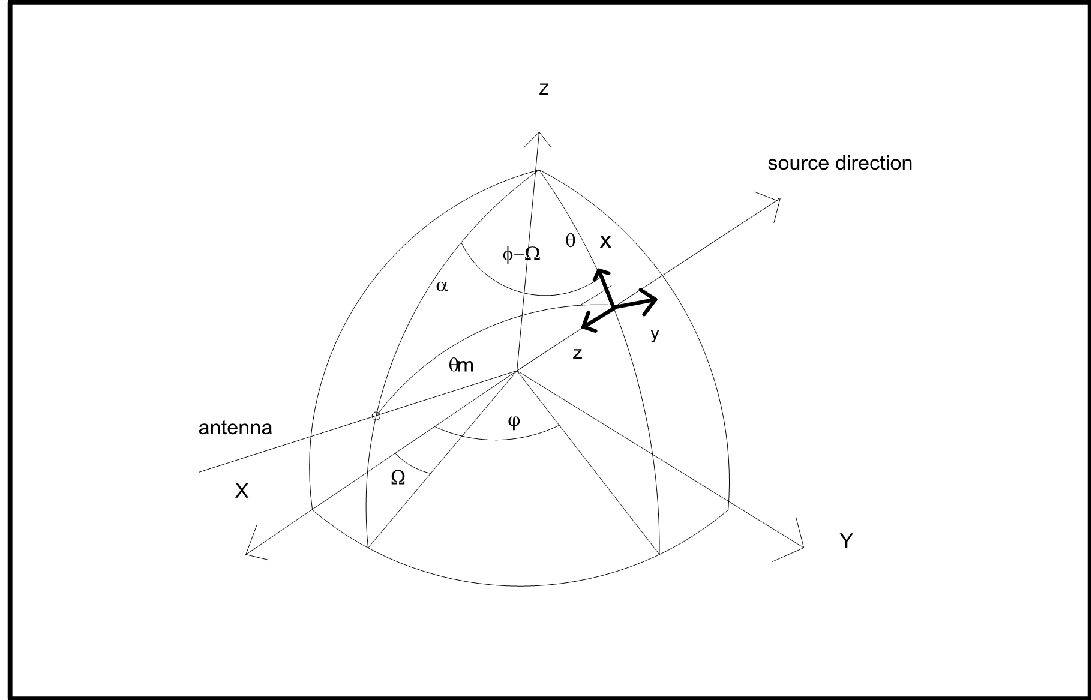
\includegraphics[width=12cm]{df_coordinate_system}
  \caption{Coordinate frame}\label{fig_coordinate_frame_DF}
\end{figure}

X, Y and Z define the spacecraft centered orthogonal cartesian coordinate system, while x,y and z define the coordinate system of the incident electromagnetic wave. The wave vector $\textbf{k}$ points in the positive z-axis, so the equation of the electric field of the wave is

\begin{equation}
\textbf{E}=\textbf{E}_0 e^{i(\textbf{k} \cdot \textbf{r} - \omega t)}
\end{equation}


The electric field is the sum of the components in x and y direction. There is no component in the z direction.

\begin{eqnarray}
\textbf{E}&=&E_x\textbf{e}_x + E_y\textbf{e}_y\\
E_x&=&E_{0,x} e^{i(kz - \omega t)} \label{Ex} \\
E_y&=&E_{0,y} e^{i(kz - \omega t - \delta)} \label{Ey}
\end{eqnarray}

$\delta$ is the phase shift between the x and y components of the E-field. The direction of the incident wave is defined by the angles $\vartheta$ and $\varphi$, the effective height vector points to the direction that is defined by the angles $\alpha$ and $\Omega$.\\

The 4 Stokes parameter define the polarization of the wave. They can be written in the following form:

\begin{equation}
S_0=I= \left\langle E_{x}^2\right\rangle +\left\langle E_{y}^2\right\rangle
\end{equation}
\begin{equation}
S_1=Q=\left\langle E_{x}^2\right\rangle-\left\langle E_{y}^2\right\rangle
\end{equation}
\begin{equation}
S_2=U=\left\langle2E_{x} E_{y} \cos \delta \right\rangle
\end{equation}
\begin{equation}
S_3=V=\left\langle2E_{x} E_{y} \sin\delta\right\rangle
\end{equation}

The Stokes Parameters are more useful in normalized form.

\begin{eqnarray}
\frac{S_0}{2\eta_0} = \hat{I} &=& \frac{\left\langle E_{x}^2\right\rangle +\left\langle E_{y}^2\right\rangle}{2\eta_0} \label{norm_stokes_1}
\\
\frac{S_1}{S_0}=\hat{Q}&=&\frac{\left\langle E_{x}^2\right\rangle-\left\langle E_{y}^2\right\rangle}{\left\langle E_{x}^2\right\rangle +\left\langle E_{y}^2\right\rangle}\label{norm_stokes_2}
\\
\frac{S_2}{S_0}=\hat{U}&=&\frac{\left\langle2E_{x} E_{y} \cos\delta\right\rangle}{\left\langle E_{x}^2\right\rangle +\left\langle E_{y}^2\right\rangle}\label{norm_stokes_3}
\\
\frac{S_3}{S_0}=\hat{V}&=&\frac{\left\langle2E_{x} E_{y} \sin\delta\right\rangle}{\left\langle E_{x}^2\right\rangle +\left\langle E_{y}^2\right\rangle}\label{norm_stokes_4}
\end{eqnarray}

The output values of the measurements are the auto- and cross-correlation parameters. For two antennas X and Z, they would be

\begin{center}
\begin{tabular}{c}
$\left\langle V_X V_X^* \right\rangle $  \\
$\left\langle V_Z V_Z^* \right\rangle $  \\
$Re\left\langle V_X V_Z^* \right\rangle $  \\
$Im\left\langle V_X V_Z^* \right\rangle $  \\
\end{tabular}
\end{center}


$V_i$ is the voltage induced in antenna i and the star means the complex conjugate. The angular brackets indicate the mean value. In general, for a complex function $C(t)$,

\begin{equation}
\left\langle CC^* \right\rangle = \frac{1}{T}\int_0^T CC^* dt
\end{equation}

This equation gives only a good result, if T is large in relation to the period of the EM wave. So the next step is to find a formula for V. The basic equation, upon which the method of direction finding is built, is

\begin{equation}
V=\textbf{l}_{eff}\cdot \textbf{E}
\end{equation}

$\textbf{l}_{eff}$ is the effective length vector. When written in component form, one can write

\begin{equation}
V=l_{eff,x} E_x + l_{eff,y} E_y \footnote{The coordinate frame is defined in a way that the electric field has no z-component.}
\end{equation}

After substituting equations (\ref{Ex}) and (\ref{Ey}) one obtains

\begin{equation}
V=l_{eff,x} E_{0,x} e^{i(kz - \omega t)}  + l_{eff,y} E_{0,y} e^{i(kz - \omega t - \delta)}
\end{equation}

If the antenna is located at $z=0$ and short in relation to the wavelength, it can be simplified.

\begin{equation}
V=l_{eff,x} E_{0,x} e^{i(\omega t)}  + l_{eff,y} E_{0,y} e^{i(\omega t - \delta)}\label{V}
\end{equation}

Hence, the next step is to find the x and y components of $\textbf{l}_{eff}$. By using the unit vector in the direction of $\textbf{l}_{eff}$, one can write

\begin{equation}
\textbf{l}_{eff} = l_{eff}\left[ \begin{array}{c}
\sin \alpha \cos \Omega\\
\sin \alpha \sin \Omega\\
\cos \alpha
\end{array}  \right]
\end{equation}

The unit vectors of the spherical coordinate system are

\begin{eqnarray}
\textbf{e}_r &=& \left[ \begin{array}{c}
\sin \theta \cos \varphi\\
\sin \theta \sin \varphi\\
\cos \theta
\end{array}  \right] \\
\textbf{e}_\theta &=& \left[ \begin{array}{c}
\cos \theta \cos \varphi\\
\cos \theta \sin \varphi\\
-\sin \theta
\end{array}  \right] \\
\textbf{e}_\varphi &=& \left[ \begin{array}{c}
-\sin  \varphi\\
\cos \varphi\\
0
\end{array}  \right]
\end{eqnarray}

By looking at Figure \ref{fig_coordinate_frame_DF}, one can easily see that the direction of the negative x-axis (small x) is also the negative $\theta$ direction  $(\textbf{e}_x=-\textbf{e}_\theta)$. Hence

\begin{equation}
{l}_{eff,x} = -l_{eff} \left[ \begin{array}{c}
\sin \alpha \cos \Omega\\
\sin \alpha \sin \Omega\\
\cos \alpha
\end{array}  \right] \cdot \left[ \begin{array}{c}
\cos \theta \cos \varphi\\
\cos \theta \sin \varphi\\
-\sin \theta
\end{array}  \right]
\end{equation}

That is

\begin{equation}
{l}_{eff,x} = l_{eff}( \sin \theta \cos \alpha - \sin \alpha \cos\theta\cos (\varphi - \Omega ) )\label{heff_x}
\end{equation}

Equivalently $\textbf{e}_y=\textbf{e}_\varphi$.

\begin{equation}
{l}_{eff,y} = l_{eff} \left[ \begin{array}{c}
\sin \alpha \cos \Omega\\
\sin \alpha \sin \Omega\\
\cos \alpha
\end{array}  \right] \cdot \left[ \begin{array}{c}
-\sin \varphi\\
\cos \varphi\\
0
\end{array}  \right]
\end{equation}

or

\begin{equation}
{l}_{eff,y} = -l_{eff}( \sin \alpha \sin (\varphi - \Omega ) )\label{heff_y}
\end{equation}


Using equations (\ref{V}), (\ref{heff_x}) and (\ref{heff_y}), one can get a general expression for the voltage which is induced in an antenna.

\begin{eqnarray}
V & = & l_{eff} [ (\sin \theta \cos \alpha - \sin \alpha \cos \theta \cos (\varphi - \Omega) )E_{0,x}e^{i \omega t} - \nonumber \\
& & -(\sin \alpha \sin (\varphi - \Omega))E_{0,y}e^{i (\omega t-\delta) } ] \nonumber \\
& = & l_{eff} e^{i \omega t} [ (\sin \theta \cos \alpha - \sin \alpha \cos \theta \cos (\varphi - \Omega) )E_{0,x} - \\
& & -(\sin \alpha \sin (\varphi - \Omega))E_{0,y}e^{-i \delta } ] \nonumber
\end{eqnarray}


This equation is valid for any monopole antenna, irrespective of its orientation as long as the frequency is low enough, such that the imaginary parts of the effective length vectors are vanishing small. To model the observables, one has to perform the necessary multiplications. For two antennas, indexed i and j, one gets

\begin{eqnarray}
V_i V_i^{*} &=& l_{eff,i}^2[E_{0,x}^2 (\sin^2 \theta \cos^2 \alpha_i -\frac{1}{2} \sin (2\alpha_i) \sin(2\theta) \cos^2(\varphi - \Omega_i) + \nonumber \\
& & + \sin^2\alpha_i \cos^2\theta \cos^2(\varphi - \Omega_i))+ \\
& & + E_{0,y}^2 \sin^2\alpha_i \sin^2 (\varphi - \Omega_i) +\nonumber \\
& & +  \frac{1}{2} E_{0,x} E_{0,y} (-\sin \theta \sin 2\alpha_i \sin(\varphi - \Omega_i) + \nonumber \\
&&+\sin^2\alpha_i \cos \theta sin(2\varphi - 2\Omega_i)) (e^{i \delta} + e^{-i \delta } )]\nonumber
\end{eqnarray}

and

\begin{eqnarray}
V_i V_j^{*} &=& l_{eff,i} l_{eff,j}[E_{0,x}^2 (\sin^2 \theta \cos \alpha_i \cos \alpha_j - \\
& & - \frac{1}{2}  \sin(2\theta) (\sin \alpha_j \cos \alpha_i \cos(\varphi - \Omega_j)+ \nonumber \\
& & +\sin \alpha_i \cos \alpha_j \cos(\varphi - \Omega_i) )+ \nonumber \\
& & + \sin \alpha_i \sin \alpha_j \cos^2\theta \cos(\varphi - \Omega_i) \cos(\varphi - \Omega_j))+ \nonumber \\
& & + E_{0,y}^2 \sin \alpha_i \sin \alpha_j \sin (\varphi - \Omega_i) \sin (\varphi - \Omega_j)\nonumber \\
& & -E_{0,x} E_{0,y} e^{i \delta}( \sin \alpha_j \sin(\varphi - \Omega_j)( \cos \alpha_i \sin \theta - \nonumber \\
& &- \sin \alpha_i \cos \theta \cos(\varphi - \Omega_i)))-\nonumber \\
& &  -E_{0,x} E_{0,y} e^{-i \delta}( \sin \alpha_i \sin(\varphi - \Omega_i)( \cos \alpha_j \sin \theta - \nonumber \\
& & -\sin \alpha_j \cos \theta \cos(\varphi - \Omega_j)))]\nonumber
\end{eqnarray}

When standardized over time

\begin{eqnarray}
\left\langle V_i V_i^{*} \right\rangle &=&  l_{eff,i}^2[\left\langle E_{0,x}^2\right\rangle (\sin^2 \theta \cos^2 \alpha_i -\nonumber\\
& & -\frac{1}{2} \sin (2\alpha_i) \sin(2\theta) \cos^2(\varphi - \Omega_i) + \\
& & + \sin^2\alpha_i \cos^2\theta \cos^2(\varphi - \Omega_i))+ \nonumber \\
& & + \left\langle E_{0,y}^2 \right\rangle \sin^2\alpha_i \sin^2 (\varphi - \Omega_i)+ \nonumber \\
& & +  \left\langle E_{0,x} E_{0,y} \cos \delta \right\rangle (-\sin \theta \sin 2\alpha_i \sin(\varphi - \Omega_i) + \nonumber \\
& &+ \sin^2\alpha_i \cos \theta sin(2\varphi - 2\Omega_i)) ]\nonumber
\end{eqnarray}

\begin{eqnarray}
Re \left\langle V_i V_j^{*}\right\rangle &=&  l_{eff,i} l_{eff,j}[\left\langle E_{0,x}^2\right\rangle (\sin^2 \theta \cos \alpha_i \cos \alpha_j - \\
& & - \frac{1}{2}  \sin(2\theta) (\sin \alpha_j \cos \alpha_i \cos(\varphi - \Omega_j)+\nonumber \\
& & \sin \alpha_i \cos \alpha_j \cos(\varphi - \Omega_i) ) + \nonumber \\
& & + \sin \alpha_i \sin \alpha_j \cos^2\theta \cos(\varphi - \Omega_i) \cos(\varphi - \Omega_j))+ \nonumber \\
& & + \left\langle E_{0,y}^2 \right\rangle \sin \alpha_i \sin \alpha_j \sin (\varphi - \Omega_i) \sin (\varphi - \Omega_j)-\nonumber \\
& & -\left\langle E_{0,x} E_{0,y} \cos\delta \right\rangle(\sin \theta(\sin \alpha_i \cos \alpha_j \sin (\varphi - \Omega_i) +  \nonumber \\
& & + \sin \alpha_j \cos \alpha_i \sin (\varphi - \Omega_j))-\nonumber \\
& & -\cos \theta \sin \alpha_i \sin \alpha_j(\sin (\varphi - \Omega_j) \cos (\varphi - \Omega_i)+ \nonumber \\
& & + \sin (\varphi - \Omega_i) \cos (\varphi - \Omega_j) ) )]\nonumber
\end{eqnarray}

\begin{eqnarray}
Im \left\langle V_i V_j^{*}\right\rangle &=& - l_{eff,i} l_{eff,j}\left\langle E_{0,x} E_{0,y} \sin \delta \right\rangle \\
& & [ (\sin \theta(\sin \alpha_i \cos \alpha_j \sin (\varphi - \Omega_i) -  \nonumber \\
& & - \sin \alpha_j \cos \alpha_i \sin (\varphi - \Omega_j))+ \nonumber \\
& & + \cos \theta \sin \alpha_i \sin \alpha_j(\sin (\varphi - \Omega_j) \cos (\varphi - \Omega_i)+ \nonumber \\
& & + \sin (\varphi - \Omega_i) \cos (\varphi - \Omega_j) ) )]\nonumber
\end{eqnarray}

When combined with (\ref{norm_stokes_1}) to (\ref{norm_stokes_4}), one gets

\begin{eqnarray}
\left\langle V_i V_i^{*} \right\rangle &=& \hat{S}\eta_0 l_{eff,i}^2[(\hat{Q}+1) (\sin^2 \theta \cos^2 \alpha_i -\\
& & -\frac{1}{2} \sin (2\alpha_i) \sin(2\theta) \cos^2(\varphi - \Omega_i) + \nonumber \\
& & + \sin^2\alpha_i \cos^2\theta \cos^2(\varphi - \Omega_i))+ \nonumber \\
& & + (1-\hat{Q}) \sin^2\alpha_i \sin^2 (\varphi - \Omega_i)+ \nonumber \\
& & +  \hat{U}  (-\sin \theta \sin 2\alpha_i \sin(\varphi - \Omega_i) +\nonumber \\
& & + \sin^2\alpha_i \cos \theta sin(2\varphi - 2\Omega_i)) ]\nonumber
\end{eqnarray}

\begin{eqnarray}
Re \left\langle V_i V_j^{*}\right\rangle &=& \hat{S}\eta_0 l_{eff,i} l_{eff,j}[(\hat{Q}+1) (\sin^2 \theta \cos \alpha_i \cos \alpha_j - \\
& & - \frac{1}{2}  \sin(2\theta) (\sin \alpha_j \cos \alpha_i \cos(\varphi - \Omega_j)+\nonumber \\
& & +\sin \alpha_i \cos \alpha_j \cos(\varphi - \Omega_i) ) + \nonumber \\
& & + \sin \alpha_i \sin \alpha_j \cos^2\theta \cos(\varphi - \Omega_i) \cos(\varphi - \Omega_j))+ \nonumber \\
& & + (1-\hat{Q}) \sin \alpha_i \sin \alpha_j \sin (\varphi - \Omega_i) \sin (\varphi - \Omega_j)-\nonumber \\
& & -\hat{U} (\sin \theta(\sin \alpha_i \cos \alpha_j \sin (\varphi - \Omega_i) +  \nonumber \\
& & + \sin \alpha_j \cos \alpha_i \sin (\varphi - \Omega_j))- \nonumber \\
& & - \cos \theta \sin \alpha_i \sin \alpha_j(\sin (\varphi - \Omega_j) \cos (\varphi - \Omega_i)+ \nonumber \\
& & + \sin (\varphi - \Omega_i) \cos (\varphi - \Omega_j) ) )]\nonumber
\end{eqnarray}

\begin{eqnarray}
Im \left\langle V_i V_j^{*}\right\rangle &=& - \hat{S}\eta_0 l_{eff,i} l_{eff,j} \hat{V}[ (\sin \theta(\sin \alpha_i \cos \alpha_j \sin (\varphi - \Omega_i) - \nonumber \\
& & - \sin \alpha_j \cos \alpha_i \sin (\varphi - \Omega_j))+  \\
& & +\cos \theta \sin \alpha_i \sin \alpha_j(\sin (\varphi - \Omega_j) \cos (\varphi - \Omega_i)+ \nonumber \\
& & + \sin (\varphi - \Omega_i) \cos (\varphi - \Omega_j) ) )]\nonumber
\end{eqnarray}

Now two substitutions yield a slightly clearer form of the equation system (see \cite{cecconi04}).

\begin{eqnarray}
A_i &=& \cos \alpha_i \sin \theta - \sin \alpha_i \cos \theta \cos (\varphi - \Omega_i)\label{A_i} \\
B_i &=& -\sin \alpha_i \sin (\varphi - \Omega_i) \label{B_i}
\end{eqnarray}

Hence:

\begin{eqnarray}
\left\langle V_i V_i^{*} \right\rangle &=& \hat{S}\eta_0 l_{eff,i}^2[(\hat{Q}+1) A^2_i + (1-\hat{Q}) B^2_i+ 2 \hat{U}A_i B_i]  \label{auto_corr_allgemein}\\
Re \left\langle V_i V_j^{*}\right\rangle &=& \hat{S}\eta_0 l_{eff,i} l_{eff,j}[(\hat{Q}+1) A_i A_j + (1-\hat{Q}) B_i B_j + \label{re_corr_allgemein}\\
& & + \hat{U} (A_i B_j + A_j B_i)] \nonumber \\
Im \left\langle V_i V_j^{*}\right\rangle &=& -\hat{S}\eta_0 l_{eff,i} l_{eff,j} \hat{V}[-A_i B_j + A_j B_i ] \label{im_corr_allgemein}
\end{eqnarray}

So for each pair of antennas, one gets a system of 3 equations with 8 unknown parameters. Clearly, with two antennas and one measurement, one cannot solve this system. With three antennas a solution exists, even an analytical one. This analytical solution will be described in the next section.

\section{The analytical solution}
\subsection{The direction of the incident wave}

As first step, the reference frame will be defined in a way that the effective length vector of the Z-antenna points in the Z-direction. Then one can refine (\ref{auto_corr_allgemein})-(\ref{im_corr_allgemein}).  When substituting the angles of the Z-antenna into (\ref{A_i}) and (\ref{B_i}), one realizes that $A_Z$ is equivalent to $sin \theta$, $B_Z$ has a value of zero.

\begin{eqnarray}
\left\langle V_Z V_Z^{*} \right\rangle &=& \hat{S}\eta_0 l_{eff,Z}^2[(\hat{Q}+1) \sin^2 \theta]   \\
Re \left\langle V_X V_Z^{*}\right\rangle &=& \hat{S}\eta_0 l_{eff,X} l_{eff,Z}[(\hat{Q}+1) (\sin^2 \theta \cos \alpha_X  - \\
& & - \frac{1}{2}  \sin(2\theta) \sin \alpha_X  \cos(\varphi - \Omega_X))  - \nonumber \\
& & -\hat{U} \sin \theta \sin \alpha_X  \sin (\varphi - \Omega_X)   ]\nonumber \\
Re \left\langle V_Y V_Z^{*}\right\rangle &=& \hat{S}\eta_0 l_{eff,Y} l_{eff,Z}[(\hat{Q}+1) (\sin^2 \theta \cos \alpha_Y  - \\
& & - \frac{1}{2}  \sin(2\theta) \sin \alpha_Y  \cos(\varphi - \Omega_Y))  - \nonumber \\
& & -\hat{U} \sin \theta \sin \alpha_Y  \sin (\varphi - \Omega_Y)   ]\nonumber \\
Im \left\langle V_X V_Z^{*}\right\rangle &=&  -\hat{S}\eta_0 l_{eff,X} l_{eff,Z} \hat{V}[ \sin \theta \sin \alpha_X  \sin (\varphi - \Omega_X) ] \\
Im \left\langle V_Y V_Z^{*}\right\rangle &=&  -\hat{S}\eta_0 l_{eff,Y} l_{eff,Z} \hat{V}[ \sin \theta \sin \alpha_Y  \sin (\varphi - \Omega_Y) ]
\end{eqnarray}


An equation for $\varphi$ can be found by using the imaginary cross-correlation-parameters.

\begin{eqnarray}
\frac{Im \left\langle V_X V_Z^{*}\right\rangle }{Im \left\langle V_Y V_Z^{*}\right\rangle}&=&\frac{- \hat{S}\eta_0 l_{eff,X} l_{eff,Z} \hat{V}[ \sin \theta \sin \alpha_X  \sin (\varphi - \Omega_X) ]}{- \hat{S}\eta_0 l_{eff,Y} l_{eff,Z} \hat{V}[ \sin \theta \sin \alpha_Y  \sin (\varphi - \Omega_Y) ] }\\
&=&\frac{l_{eff,X}}{l_{eff,Y}}\frac{ \sin \alpha_X  \sin (\varphi - \Omega_X) }{ \sin \alpha_Y  \sin (\varphi - \Omega_Y)  }\\
&=&\frac{l_{eff,X} \sin \alpha_X}{l_{eff,Y} \sin \alpha_Y}\frac{(\tan \varphi -\tan \Omega_X)  \cos \varphi \cos \Omega_X}{( \tan \varphi -\tan \Omega_Y) \cos \varphi \cos  \Omega_Y  }\\
&=&\frac{l_{eff,X} \sin \alpha_X}{l_{eff,Y} \sin \alpha_Y}\frac{(\tan \varphi -\tan \Omega_X)  \cos \Omega_X}{( \tan \varphi -\tan \Omega_Y) \cos  \Omega_Y  } \\
&=&\frac{l_{eff,X} \sin \alpha_X}{l_{eff,Y} \sin \alpha_Y}\frac{(\tan \varphi \cos \Omega_X-\tan \Omega_X \cos \Omega_X) }{( \tan \varphi \cos \Omega_Y-\tan \Omega_Y \cos \Omega_Y) }
\end{eqnarray}

Hence :

\begin{eqnarray}
& & Im \left\langle V_X V_Z^{*}\right\rangle l_{eff,Y} \sin \alpha_Y ( \tan \varphi \cos \Omega_Y-\tan \Omega_Y \cos \Omega_Y) \\
&=& Im \left\langle V_Y V_Z^{*}\right\rangle l_{eff,X} \sin \alpha_X (\tan \varphi \cos \Omega_X-\tan \Omega_X \cos \Omega_X) \nonumber
\end{eqnarray}

or

\begin{eqnarray}
 Im \left\langle V_X V_Z^{*}\right\rangle l_{eff,Y} \sin \alpha_Y \tan \varphi \cos \Omega_Y - & &\\
 -Im \left\langle V_X V_Z^{*}\right\rangle l_{eff,Y} \sin \alpha_Y \tan \Omega_Y \cos \Omega_Y &=&\nonumber\\
 Im \left\langle V_Y V_Z^{*}\right\rangle l_{eff,X} \sin \alpha_X \tan \varphi \cos \Omega_X - & &\nonumber \\
 -Im \left\langle V_Y V_Z^{*}\right\rangle l_{eff,X} \sin \alpha_X \tan \Omega_X \cos \Omega_X & &\nonumber
\end{eqnarray}

\begin{eqnarray}
 Im \left\langle V_X V_Z^{*}\right\rangle l_{eff,Y} \sin \alpha_Y \tan \varphi \cos \Omega_Y-& &\\
 -Im \left\langle V_Y V_Z^{*}\right\rangle l_{eff,X} \sin \alpha_X \tan \varphi \cos \Omega_X &=&\nonumber \\
 Im \left\langle V_X V_Z^{*}\right\rangle l_{eff,Y} \sin \alpha_Y \tan \Omega_Y \cos \Omega_Y - & &\nonumber\\
 -Im \left\langle V_Y V_Z^{*}\right\rangle l_{eff,X} \sin \alpha_X \tan \Omega_X \cos \Omega_X & &\nonumber
\end{eqnarray}

\begin{eqnarray}
\tan \varphi  (Im \left\langle V_X V_Z^{*}\right\rangle l_{eff,Y} \sin \alpha_Y \cos \Omega_Y-& &\\
 -Im \left\langle V_Y V_Z^{*}\right\rangle l_{eff,X} \sin \alpha_X  \cos \Omega_X) &=&\nonumber \\
 Im \left\langle V_X V_Z^{*}\right\rangle l_{eff,Y} \sin \alpha_Y \tan \Omega_Y \cos \Omega_Y -& &\nonumber\\
 -Im \left\langle V_Y V_Z^{*}\right\rangle l_{eff,X} \sin \alpha_X \tan \Omega_X \cos \Omega_X & &\nonumber
\end{eqnarray}

\begin{eqnarray}\label{tan_phi}
\tan \varphi &=& [Im \left\langle V_X V_Z^{*}\right\rangle l_{eff,Y} \sin \alpha_Y \tan \Omega_Y \cos \Omega_Y-\\
& & -Im \left\langle V_Y V_Z^{*}\right\rangle l_{eff,X} \sin \alpha_X \tan \Omega_X \cos \Omega_X] \times \nonumber \\
& &\times[Im \left\langle V_X V_Z^{*}\right\rangle l_{eff,Y} \sin \alpha_Y \cos \Omega_Y -\nonumber \\
& &  -Im \left\langle V_Y V_Z^{*}\right\rangle l_{eff,X} \sin \alpha_X  \cos \Omega_X]^{-1}\nonumber
\end{eqnarray}

The right hand side contains only known parameters, so one can get an analytical solution of the azimuth of the incident wave. The tangent function is unambiguous only over a range of $\pi$, so one has to know or guess in advance, from where the radiation approximately arrives. Also the colatitude can be determined analytically. One has to employ the equations of $\left\langle V_Z V_Z^{*} \right\rangle$, $Re \left\langle V_X V_Z^{*}\right\rangle$ and $Re \left\langle V_Y V_Z^{*}\right\rangle$ for this purpose. At first the real parts of the cross-correlation-parameters are multiplied by the respective factors, such that the last term of the equations vanish by subtraction.

\begin{eqnarray}
&&Re \left\langle V_X V_Z^{*}\right\rangle \sin \alpha_Y  \sin (\varphi - \Omega_Y)l_{eff,Y} = \\
&=& \hat{S}\eta_0  l_{eff,Z}[(\hat{Q}+1) l_{eff,X} l_{eff,Y}
(\sin^2 \theta \cos \alpha_X  \sin \alpha_Y  \sin (\varphi - \Omega_Y) - \nonumber \\
&& - \frac{1}{2}  \sin(2\theta) \sin \alpha_X  \sin \alpha_Y \cos(\varphi - \Omega_X)  \sin (\varphi - \Omega_Y) )  - \nonumber \\
&& -\hat{U} \sin \theta \sin \alpha_X  \sin \alpha_Y  \sin (\varphi - \Omega_X)  \sin (\varphi - \Omega_Y) l_{eff,X} l_{eff,Y}  ] \nonumber
\end{eqnarray}

\begin{eqnarray}
&&Re \left\langle V_Y V_Z^{*}\right\rangle\sin \alpha_X  \sin (\varphi - \Omega_X) l_{eff,X}=  \\
&=& \hat{S}\eta_0 l_{eff,Z}[(\hat{Q}+1)l_{eff,X} l_{eff,Y}  (\sin^2 \theta \cos \alpha_Y \sin \alpha_X  \sin (\varphi - \Omega_X) -\nonumber \\
&& - \frac{1}{2}  \sin(2\theta) \sin \alpha_X \sin \alpha_Y  \cos(\varphi - \Omega_Y)  \sin (\varphi - \Omega_X))  - \nonumber \\
&& -\hat{U} \sin \theta \sin \alpha_X \sin \alpha_Y  \sin (\varphi - \Omega_X) \sin (\varphi - \Omega_Y) l_{eff,X} l_{eff,Y}    ]\nonumber
\end{eqnarray}

Now the equations can be subtracted.

\begin{eqnarray}
&&Re \left\langle V_X V_Z^{*}\right\rangle \sin \alpha_Y  \sin (\varphi - \Omega_Y) l_{eff,Y}
-\nonumber \\
&&- Re \left\langle V_Y V_Z^{*}\right\rangle\sin \alpha_X  \sin (\varphi - \Omega_X) l_{eff,X}= \nonumber\\
&=& \hat{S}\eta_0  l_{eff,Z}[(\hat{Q}+1) l_{eff,X} l_{eff,Y} (  \sin^2 \theta ( \cos \alpha_X  \sin \alpha_Y  \sin (\varphi - \Omega_Y)-\nonumber \\
&& -\cos \alpha_Y \sin \alpha_X  \sin (\varphi - \Omega_X))+\nonumber \\
&& \sin \theta \cos \theta \sin \alpha_X  \sin \alpha_Y ( \cos (\varphi - \Omega_Y)  \sin (\varphi - \Omega_X)-\nonumber \\
&& -\cos (\varphi - \Omega_X)  \sin (\varphi - \Omega_Y)) ]
\end{eqnarray}

Then the equation are divided by $\left\langle V_Z V_Z^{*} \right\rangle$.

\begin{eqnarray}
&&[Re \left\langle V_X V_Z^{*}\right\rangle \sin \alpha_Y  \sin (\varphi - \Omega_Y) l_{eff,Y}-\nonumber \\
&&-Re \left\langle V_Y V_Z^{*}\right\rangle\sin \alpha_X  \sin (\varphi - \Omega_X) l_{eff,X}] \left[ \left\langle V_Z V_Z^{*} \right\rangle \right]^{-1} =\nonumber \\
&=&[\hat{S}\eta_0  l_{eff,Z}[(\hat{Q}+1) l_{eff,X} l_{eff,Y} (  \sin^2 \theta ( \cos \alpha_X  \sin \alpha_Y  \sin (\varphi - \Omega_Y)-\nonumber \\
&& - \cos \alpha_Y \sin \alpha_X  \sin (\varphi - \Omega_X)) +\nonumber \\
&&+ \sin \theta \cos \theta \sin \alpha_X  \sin \alpha_Y ( \cos (\varphi - \Omega_Y)  \sin (\varphi - \Omega_X)-\nonumber \\
&&- \cos (\varphi - \Omega_X)  \sin (\varphi - \Omega_Y)) ]][\hat{S}\eta_0 h_{eff,Z}^2[(\hat{Q}+1) \sin^2 \theta ]]^{-1}
\end{eqnarray}

\begin{eqnarray}
&&[Re \left\langle V_X V_Z^{*}\right\rangle \sin \alpha_Y  \sin (\varphi - \Omega_Y) l_{eff,Y}-\nonumber \\
&&-Re \left\langle V_Y V_Z^{*}\right\rangle\sin \alpha_X  \sin (\varphi - \Omega_X) l_{eff,X}] \left[ \left\langle V_Z V_Z^{*} \right\rangle \right] ^{-1}= \nonumber \\
&&= \frac{  l_{eff,X} l_{eff,Y}}{ l_{eff,Z}} [\cos \alpha_X  \sin \alpha_Y  \sin (\varphi - \Omega_Y)  \nonumber\\
&&- \cos \alpha_Y \sin \alpha_X  \sin (\varphi - \Omega_X) +\nonumber \\
&&+  \frac{\cos \theta}{\sin \theta\ } \sin \alpha_X  \sin \alpha_Y ( \cos (\varphi - \Omega_Y)  \sin (\varphi - \Omega_X)-\nonumber \\
&&- \cos (\varphi - \Omega_X)  \sin (\varphi - \Omega_Y)) ]
\end{eqnarray}

\begin{eqnarray}
&&Re \left\langle V_X V_Z^{*}\right\rangle \sin \alpha_Y  \sin (\varphi - \Omega_Y) l_{eff,Y}l_{eff,Z}-\nonumber \\
&&-Re \left\langle V_Y V_Z^{*}\right\rangle\sin \alpha_X  \sin (\varphi - \Omega_X) l_{eff,X}l_{eff,Z}= \nonumber \\
&=&\left\langle V_Z V_Z^{*} \right\rangle l_{eff,X} l_{eff,Y} [\cos \alpha_X  \sin \alpha_Y  \sin (\varphi - \Omega_Y)- \nonumber \\
&&- \cos \alpha_Y \sin \alpha_X  \sin (\varphi - \Omega_X) + \nonumber \\
&&+  \frac{1}{\tan \theta\ } \sin \alpha_X  \sin \alpha_Y ( \cos (\varphi - \Omega_Y)  \sin (\varphi - \Omega_X)- \nonumber \\
&&-\cos (\varphi - \Omega_X)  \sin (\varphi - \Omega_Y)) ]
\end{eqnarray}

Now the analytical solution for the colatitude $\theta$  is in close reach.

\begin{eqnarray}
&&[Re \left\langle V_X V_Z^{*}\right\rangle \sin \alpha_Y  \sin (\varphi - \Omega_Y) l_{eff,Y}l_{eff,Z}-\nonumber \\
&&-Re \left\langle V_Y V_Z^{*}\right\rangle\sin \alpha_X  \sin (\varphi - \Omega_X) l_{eff,X}l_{eff,Z}]\times \nonumber \\
&& \times \left[ \left\langle V_Z V_Z^{*} \right\rangle l_{eff,X} l_{eff,Y} \right]^{-1} =\nonumber \\
&=& \cos \alpha_X  \sin \alpha_Y  \sin (\varphi - \Omega_Y)-  \cos \alpha_Y \sin \alpha_X  \sin (\varphi - \Omega_X) +\nonumber \\
&&+  \frac{1}{\tan \theta\ } \sin \alpha_X  \sin \alpha_Y ( \cos (\varphi - \Omega_Y)  \sin (\varphi - \Omega_X)-\nonumber \\
&&- \cos (\varphi - \Omega_X)  \sin (\varphi - \Omega_Y))
\end{eqnarray}

\begin{eqnarray}
&&[Re \left\langle V_X V_Z^{*}\right\rangle \sin \alpha_Y  \sin (\varphi - \Omega_Y) l_{eff,Y}l_{eff,Z}-\nonumber \\
&&-Re\left\langle V_Y V_Z^{*}\right\rangle\sin \alpha_X  \sin (\varphi - \Omega_X) l_{eff,X}l_{eff,Z}]\times \nonumber \\
&&\times \left[ \left\langle V_Z V_Z^{*} \right\rangle l_{eff,X} l_{eff,Y}\right]^{-1}+\nonumber \\
&&+\cos \alpha_Y \sin \alpha_X  \sin (\varphi - \Omega_X)-\cos \alpha_X  \sin \alpha_Y  \sin (\varphi - \Omega_Y)=\nonumber \\
&=&  \frac{1}{\tan \theta\ } \sin \alpha_X  \sin \alpha_Y ( \cos (\varphi - \Omega_Y)  \sin (\varphi - \Omega_X) - \nonumber \\
&&-\cos (\varphi - \Omega_X)  \sin (\varphi - \Omega_Y))
\end{eqnarray}

\begin{eqnarray}
&&\left[ \tan \theta \right]  \times [ \sin \alpha_X  \sin \alpha_Y ( \cos (\varphi - \Omega_Y)  \sin (\varphi - \Omega_X)-\nonumber \\
&&-\cos (\varphi - \Omega_X)  \sin (\varphi - \Omega_Y))]^{-1} = \nonumber \\
&=& [\left\langle V_Z V_Z^{*} \right\rangle l_{eff,X} l_{eff,Y}]  [Re \left\langle V_X V_Z^{*}\right\rangle \sin \alpha_Y  \sin (\varphi - \Omega_Y) l_{eff,Y}l_{eff,Z}\nonumber \\
&&-Re\left\langle V_Y V_Z^{*}\right\rangle\sin \alpha_X  \sin (\varphi - \Omega_X) l_{eff,X}l_{eff,Z} +\left\langle V_Z V_Z^{*} \right\rangle l_{eff,X} l_{eff,Y} \nonumber \\
&&\times(\cos \alpha_Y \sin \alpha_X  \sin (\varphi - \Omega_X)-\cos \alpha_X  \sin \alpha_Y  \sin (\varphi - \Omega_Y))]^{-1}
\end{eqnarray}

\begin{eqnarray}\label{tan_theta}
\tan \theta\  &=&
[\left\langle V_Z V_Z^{*} \right\rangle l_{eff,X} l_{eff,Y} \sin \alpha_X  \sin \alpha_Y \\
&\times&( \cos (\varphi - \Omega_Y)  \sin (\varphi - \Omega_X) -\cos (\varphi - \Omega_X)  \sin (\varphi - \Omega_Y))]\nonumber \\
&\times& [Re \left\langle V_X V_Z^{*}\right\rangle \sin \alpha_Y  \sin (\varphi - \Omega_Y) l_{eff,Y}l_{eff,Z} \nonumber \\
&-&Re\left\langle V_Y V_Z^{*}\right\rangle\sin \alpha_X  \sin (\varphi - \Omega_X) l_{eff,X}l_{eff,Z}\nonumber \\
&+&\left\langle V_Z V_Z^{*} \right\rangle l_{eff,X} l_{eff,Y} \nonumber \\
&\times&(\cos \alpha_Y \sin \alpha_X  \sin (\varphi - \Omega_X)-\cos \alpha_X  \sin \alpha_Y  \sin (\varphi - \Omega_Y))]^{-1} \nonumber
\end{eqnarray}

The tangent, as well as the colatitude is defined over a range of $\pi$. Hence, $\theta$ is uniquely determined.

\subsection{The Stokes parameters}

To find an analytical solution for the Stokes parameters one can use equations (\ref{auto_corr_allgemein}) to (\ref{im_corr_allgemein}). Parameters A and B are now known, due to the analysis of the recent section. For this reason, it is possible to set up a linear matrix equation by using the parameters of two antennas. The method I will show is similar to the one of Cecconi as described in \cite{cecconi04}, with the exception that it is not necessary that the X and Y antennas are located symmetrically about the X axis. The only requirement is that $l_{eff,X}$  points in the +Z direction. So, at first one needs the formulas of two antennas, e.g. X and Z.

\begin{eqnarray}
\left\langle V_X V_X^{*} \right\rangle &=& \hat{S}\eta_0 l_{eff,X}^2[(\hat{Q}+1) A^2_X   \\
&&+ (1-\hat{Q}) B^2_X+ 2 \hat{U}A_X B_X]  \nonumber \\
\left\langle V_Z V_Z^{*} \right\rangle &=& \hat{S}\eta_0 l_{eff,Z}^2[(\hat{Q}+1) A^2_Z   \\
&& + (1-\hat{Q}) B^2_Z+ 2 \hat{U}A_Z B_Z]  \nonumber \\
Re \left\langle V_X V_Z^{*}\right\rangle &=& \hat{S}\eta_0 l_{eff,X} l_{eff,Z}[(\hat{Q}+1) A_X A_Z +\\
&&+  (1-\hat{Q}) B_X B_Z + \hat{U} (A_X B_Z + A_Z B_X)] \nonumber \\
Im \left\langle V_X V_Z^{*}\right\rangle &=& -\hat{S}\eta_0 l_{eff,X} l_{eff,Z} \hat{V}[-A_X B_Z + A_Z B_X ]
\end{eqnarray}

This system can be transformed step by step.

\begin{eqnarray}
\left\langle V_X V_X^{*} \right\rangle &=& \hat{S}\eta_0 l_{eff,X}^2[\hat{Q}A^2_X+A^2_X + B^2_X \\
&&-\hat{Q} B^2_X+ 2 \hat{U}A_X B_X] \nonumber  \\
\left\langle V_Z V_Z^{*} \right\rangle &=& \hat{S}\eta_0 l_{eff,Z}^2[\hat{Q}A^2_Z+A^2_Z + B^2_Z\\
&&-\hat{Q} B^2_Z+ 2 \hat{U}A_Z B_Z]  \nonumber \\
Re \left\langle V_X V_Z^{*}\right\rangle &=& \hat{S}\eta_0 l_{eff,X} l_{eff,Z}[\hat{Q}A_X A_Z+ A_X A_Z  \\
&&+  B_X B_Z-\hat{Q} B_X B_Z +  \hat{U} (A_X B_Z + A_Z B_X)] \nonumber \\
Im \left\langle V_X V_Z^{*}\right\rangle &=& -\hat{S}\eta_0 l_{eff,X} l_{eff,Z} \hat{V}[-A_X B_Z + A_Z B_X ]
\end{eqnarray}

\begin{eqnarray}
\frac{\left\langle V_X V_X^{*} \right\rangle }{\eta_0 l_{eff,X}^2}&=& \hat{S}\hat{Q}A^2_X+\hat{S}A^2_X + \hat{S}B^2_X\\
&&-\hat{S}\hat{Q} B^2_X+ 2 \hat{S}\hat{U}A_X B_X \nonumber \\
\frac{\left\langle V_Z V_Z^{*} \right\rangle }{\eta_0 l_{eff,Z}^2}&=& \hat{S}\hat{Q}A^2_Z+\hat{S}A^2_Z + \hat{S}B^2_Z\\
&&-\hat{S}\hat{Q} B^2_Z+ 2 \hat{S}\hat{U}A_Z B_Z   \nonumber \\
\frac{Re \left\langle V_X V_Z^{*}\right\rangle }{\eta_0 l_{eff,X} l_{eff,Z}}&=& \hat{S}\hat{Q}A_X A_Z+ \hat{S}A_X A_Z +  \hat{S}B_X B_Z\\
&&-\hat{S}\hat{Q} B_X B_Z + \hat{S}\hat{U} (A_X B_Z + A_Z B_X)] \nonumber \\
\frac{Im \left\langle V_X V_Z^{*}\right\rangle }{\eta_0 l_{eff,X} l_{eff,Z}}&=& -\hat{S} \hat{V}[-A_X B_Z + A_Z B_X ]
\end{eqnarray}

\begin{eqnarray}
\frac{\left\langle V_X V_X^{*} \right\rangle }{\eta_0 l_{eff,X}^2}&=& \hat{S}(A^2_X+ B^2_X) \\
&&+\hat{S}\hat{Q}(A^2_X- B^2_X)+ 2 \hat{S}\hat{U}A_X B_X   \nonumber \\
\frac{\left\langle V_Z V_Z^{*} \right\rangle }{\eta_0 l_{eff,Z}^2}&=& \hat{S}(A^2_Z + B^2_Z) \\
&&+\hat{S}\hat{Q}(A^2_Z - B^2_Z)+ 2 \hat{S}\hat{U}A_Z B_Z   \nonumber \\
\frac{Re \left\langle V_X V_Z^{*}\right\rangle }{\eta_0 l_{eff,X} l_{eff,Z}}&=& \hat{S}(A_X A_Z +  B_X B_Z) \\
&&+ \hat{S}\hat{Q}(A_X A_Z -B_X B_Z)  \nonumber\\
&&+ \hat{S}\hat{U} (A_X B_Z + A_Z B_X)] \nonumber \\
\frac{Im \left\langle V_X V_Z^{*}\right\rangle }{\eta_0 l_{eff,X} l_{eff,Z}}&=& -\hat{S} \hat{V}(-A_X B_Z + A_Z B_X )
\end{eqnarray}

In matrix notation, one can write:

\begin{equation}\label{lineare_gleichung}
\textbf{M}\textbf{x}=\textbf{b}
\end{equation}


with

\begin{equation}
\textbf{b}=\left[ \begin{array}{c}
\frac{\left\langle V_X V_X^{*} \right\rangle }{\eta_0 l_{eff,X}^2} \\ \\
 \frac{\left\langle V_Z V_Z^{*} \right\rangle }{\eta_0 l_{eff,Z}^2}\\ \\
\frac{Re \left\langle V_X V_Z^{*}\right\rangle }{\eta_0 l_{eff,X} l_{eff,Z}} \\ \\
\frac{Im \left\langle V_X V_Z^{*}\right\rangle }{\eta_0 l_{eff,X} l_{eff,Z}}
\end{array}  \right]
\end{equation}

\begin{equation}
\textbf{x}=\left[ \begin{array}{c}
\hat{S}\\
\hat{S}\hat{Q}\\
\hat{S}\hat{U}\\
\hat{S}\hat{V}
\end{array}  \right]
\end{equation}

\tiny
\begin{equation}
\textbf{M}= \left[
\begin{array}{cccc}
(A^2_X+ B^2_X) & (A^2_X- B^2_X) & 2 A_X B_X & 0 \\
(A^2_Z+ B^2_Z) &(A^2_Z- B^2_Z)  & 2 A_Z B_Z & 0 \\
 (A_X A_Z +  B_X B_Z)& (A_X A_Z - B_X B_Z) & (A_X B_Z + A_Z B_X) & 0 \\
0 & 0 & 0 & -(-A_X B_Z + A_Z B_X )
\end{array} \right]
\end{equation}
\normalsize

This equation is solvable, as long as \textbf{M} is not singular.


\chapter{Calibration methods}
\section{Experimental methods}
\subsection{Rheometry}
\subsection{The anechoic chamber}
\section{Numerical methods}
\subsection{The Method of Moments}
The Method of Moments (MoM) is a method to solve equations which can be expressed in the language of linear spaces in the form

\begin{equation}\label{eq:linear_operator}
 L(j)=g
\end{equation}

where L is a linear operator acting on a function j, which is the response to an excitation represented by g. The MoM can be applied to many differential and integral equations in the field of mechanics, electrodynamics and other areas of physics. In the case of the application on scattering problems, the excitation usually corresponds to the electric field or voltage and the response functions j are representing the current density. The core of the MoM is that the equation is converted into a matrix equation which can be solved algebraically.\\

At first an inner product $\left\langle f,g\right\rangle$ has to be defined which has to fulfill certain requirements which originate from the theory of linear spaces and can be reviewed in respective literature.\\

The integral equation, which needs to be solved for the purpose antenna calibration is some equation which governs the behavior of electromagnetic fields, i.e. some kind of scattering equation. Common forms are the Magnetic Field Integral Equation (EFIE), the Magnetic Field Integral Equation (MFIE), the Mixed Integral Equation (MIE) and the Reaction Integral Equation (RIE). For the MoM the response function, which is the function governing the current distribution in this context, has to be approximated with a series expansion.

\begin{equation}\label{eq:bas_funct_expans}
 \mathbf{j}=\sum_{n} c_n j_n
\end{equation}

$j_n$ is called the basis function. Different kinds of functions can be used as basis functions in electromagnetic problems. The most simple function is the pulse function. A very common choice is to use linear triangular functions, which converge faster during the solution process, while other solvers use a sum of a sine and a cosine function which have the advantage of being able to be integrated analytically over the wire grid. The very well known open source software NEC 2 and NEC 4 use the sum of a sine, a cosine and a constant function. Other solutions are possible.\\

The correct choice of the basis functions is vital for the successful computation of electromagnetic problems and depends also on the area of application. When the wavelength is much longer than the typical extension of one basis function, there is little difference between usability of the three possible basis functions (pulse, linear, sinusoidal).\\

$c_n$ are the constants which are to be determined in the solution process, often called amplitudes. Combining (\ref{eq:linear_operator}) and (\ref{eq:bas_funct_expans}) gives

\begin{equation}\label{eq:expanded_func}
 \sum_{n} c_n L j_n=g
\end{equation}

Then a weighting or testing function $w_m$ has to be defined. The functions have to span the range of L, which means that also the ranges of the induces n and m are equal. Many different testing functions are suitable and in use, for instance the point function $w_m=\delta(x-x_m)$, where $x_m$ is the midpoint of wire m. This particular selection of the testing function facilitates the solution of the integral along the wire and is also used in one of the solvers implemented for this paper. An other widely used method is Galerkin's method \cite{harrington}, where the testing function is equal to the expansion function.\\


The inner product with equation (\ref{eq:expanded_func}) is formed.

\begin{equation}
 \sum_{n} c_n \left\langle w_m, L j_n\right\rangle = \left\langle w_m, g \right\rangle
\end{equation}

As matrix equation this can be written as

\begin{equation}
 l_{mn}c_n=g_m
\end{equation}

The solution for the amplitude vector is

\begin{equation}
 c_n=l_{mn}^{-1}g_m
\end{equation}

with $l_{mn}^{-1}$ being the inverse of the matrix built from the elements $l_{mn}=\left\langle w_m, L j_n\right\rangle$.\\

The resulting matrix equation has then the form


\begin{equation}\label{eq:mom}
- \mathbf{V}=\mathbf{ZC}
\end{equation}

where $Z=l_{mn}$ can be seen as an impedance. The unknown quantity is the current vector $\mathbf{C}$. \\

The excitation of the antenna system is manifested in the shape of the excitation vector $\mathbf{V}$ which was denoted $g_m$ in the general case and has the physical unit volts. When the antenna is excited at a single feed, like in the case of the spacecraft antenna calibration, all elements of the vector are set to zero, except the element corresponding to the segment which is used as feeding point in the simulation. This element is set to the excitation voltage of the antenna.\\


When the antenna system is excited by an incoming wave, the elements of the vector hold the values

\begin{equation}
 V_i=\mathbf{E(r_\mathit{i})} \cdot \mathbf{s_\mathit{i}}
\end{equation}

where $\mathbf{s_\mathit{i}}$ is the corresponding segment \textit{i} and $\mathbf{E(r_\mathit{i})}$ is the incident electric field at location $\mathbf{r}_\mathit{i}$, the location of the midpoint of segment \textit{i}.


\subsection{The Finite Difference Time Domain method}
The Finite Difference Time Domain (FDTD) method belongs, contrary to the MoM, to the family of time domain methods, so the Maxwell equations in differential and time domain form are directly solved for multiple points of space and time, which would be equations \ref{maxwell1}-\ref{maxwell4} for a linear, isotropic and non-dispersive medium. The medium is defined by the values of the permeability, permittivity and conductivity.\\

The FDTD method solves the system of equations iteratively and numerically by using a Taylor expansion and discretized spatial derivatives. The geometry of the points in space where the equations are solved, is called Yee cell (see figure \ref{fig:yee}).\\

Electric and magnetic field components are computed at different points in space and time. This has the effect of facilitating the numerical computation of the curl. There is a time difference of a half step size between the time of the values of the electric field components and the magnetic field components. This is called leap-frog scheme.\\


\begin{figure}
\begin{center}
 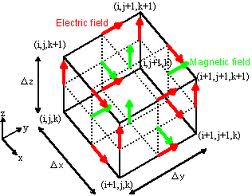
\includegraphics[width=6cm]{yee}
\caption{Yee cell}
\label{fig:yee}
\end{center}
\end{figure}

The governing equations are

\begin{eqnarray}
H_x^m(i,j,k)&=&	H_x^{m-1}(i,j,k) + \frac{\Delta t}{\mu_0 \Delta z}[ E_y^{n}(i,j,k)-E_y^{n}(i,j,k-1)]	\nonumber \\
&& -  \frac{\Delta t}{\mu_0 \Delta y}[ E_z^{n}(i,j,k)-E_z^{n}(i,j-1,k)]	\\
H_y^m(i,j,k)&=&	H_y^{m-1}(i,j,k) + \frac{\Delta t}{\mu_0 \Delta x}[E_z^{n}(i,j,k)-E_z^{n}(i-1,j,k)]	\nonumber \\
&& -  \frac{\Delta t}{\mu_0 \Delta z}[ E_x^{n}(i,j,k)-E_x^{n}(i,j,k-1)]	\\
H_z^m(i,j,k)&=&	H_z^{m-1}(i,j,k) + \frac{\Delta t}{\mu_0 \Delta y}[E_x^{n}(i,j,k)-E_x^{n}(i,j-1,k)]	\nonumber \\
&& - \frac{\Delta t}{\mu_0 \Delta x}[ E_y^{n}(i,j,k)-E_y^{n}(i-1,j,k)]	\\
E_x^n(i,j,k)&=&	\frac{2\epsilon-\sigma \Delta t}{2\epsilon+\sigma \Delta t} E_x^{n-1}(i,j,k) 	\\
&& - \frac{2\Delta t}{(2\epsilon+\sigma \Delta t)\Delta z} [H_y^m(i,j,k) - H_y^m(i,j,k-1)]	\nonumber \\
&& + \frac{2\Delta t}{(2\epsilon+\sigma \Delta t)\Delta y} [H_z^m(i,j,k) - H_z^m(i,j-1,k)]	\\
E_y^n(i,j,k)&=&	\frac{2\epsilon-\sigma \Delta t}{2\epsilon+\sigma \Delta t} E_y^{n-1}(i,j,k) 	\\
&& - \frac{2\Delta t}{(2\epsilon+\sigma \Delta t)\Delta x} [H_z^m(i,j,k) - H_z^m(i-1,j,k)]	\nonumber \\
&& + \frac{2\Delta t}{(2\epsilon+\sigma \Delta t)\Delta z} [H_x^m(i,j,k) - H_x^m(i,j,k-1)]	\\
E_z^n(i,j,k)&=&	\frac{2\epsilon-\sigma \Delta t}{2\epsilon+\sigma \Delta t} E_z^{n-1}(i,j,k) 	\\
&& - \frac{2\Delta t}{(2\epsilon+\sigma \Delta t)\Delta y} [H_x^m(i,j,k) - H_x^m(i,j-1,k)]	\nonumber \\
&& + \frac{2\Delta t}{(2\epsilon+\sigma \Delta t)\Delta x} [H_y^m(i,j,k) - H_y^m(i-1,j,k)]	
\end{eqnarray}

$\Delta x$, $\Delta y$ and $\Delta z$ are the spatial steps, $\Delta t$ the temporal. $\{i,j,k\}$ are the indices in the x-,y- and z-direction, while n and m are the temporal indices. Due to the leap frog scheme, $m=n+\frac{1}{2}$. A Yee cell has the volume $\Delta x \Delta y \Delta z$. Inside a cell, the material constants are assumed to have the same value. The positions where the field components are evaluated, are organized in a way that the rotation elements can be computed with minimum effort.\\

Voltages and currents can be computed directly from the fields, when needed, by using the respective Maxwell equations:

\begin{equation}
V_z(i,j,k)=-E_z(i,j,k) \Delta z 
\end{equation}

and

\begin{eqnarray}
I_z(i,j,k)&=& [H_x(i,j-1,k)-H_x(i,j,k)] \Delta x \\
&+&  [H_y(i,j,k)-H_y(i-1,j,k)] \Delta y
\end{eqnarray}

One of the advantages of this method is that a whole frequency spectrum can be calculated in a single computation. An impulse is synthesized from all frequencies of interest and this impulse is used as source of the calculation. The resulting field at the point of interest is analyzed by a Fourier analytical method.\\

Surfaces and bodies are simulated by setting the material constants for the Yee cells, which occupy the region in space, where the body is located, and by holding the field values at a given value, where appropriate. For instance a conducting surface has the property, that it has a constant electric potential. So to simulate a conducting body, the electric field components at the Yee cells which represent its surface, is set to 0 in the directions of the surface. For instance, a wire in the x-direction would be realized by:

\begin{eqnarray}
E_x(i,j,k)&=&0 \\
E_x(i+1,j,k)&=&0\\ 
E_x(i+2,j,k)&=&0 
\end{eqnarray}

A disadvantage of this method is, that the volume, which is included in the simulation, is always finite and the required amount of calculations increases rapidly with increasing volume. Hence, when an infinite volume is considered, for instance a calculation of an antenna in free space, a special procedure has to be used. This procedure is called near- to farfield converter. At the boundary of the volume, the incident fields are converted to far fields. The boundary has the property of absorbing all radiation as it would be when it would be the boundary to the rest of the infinite space, i.e. there are no reflections at a virtual boundary.\\

To compute the farfields, the virtual currents are at the boundary are computed, which would be induced by the fields, if the boundaries where real. Then the farfields created by these currents are computed.\\

This method is well suited for antenna in plasma calculations because, when plasma is modeled as dielectric medium, the resulting material constants can directly be used in the simulation. Also magnetized plasma can be simulated this way, much easier than with the MoM.

\subsection{The Finite Element Method}
\section{Inflight calibration}

\begin{thebibliography}{}


\bibitem[{\textit{Bale}(2008)}]{bale08}
Bale, S.D. and Ullrich, R. and Goetz, K. and Alster, N. and Cecconi, B. and Dekkali, M. and Lingner, N.R. and Macher, W. and Manning, R.E. and McCauley, J. and Monson, S.J. and Oswald, T.H. and Pulupa, M. (2008), The Electric Antennas for the STEREO/WAVES Experiment, \textit{Space Science Reviews,
doi:10.1007/s11214-007-9251-x}.

\bibitem[{\textit{Cecconi and Zarka}(2004)}]{cecconi04}
Cecconi, B., and P.~Zarka (2005), Direction finding and antenna calibration
  through analytical inversion of radio measurements performed using a system
  of 2 or 3 electric dipole wire antennas on a 3 axes stabelized spacecraft,
  \textit{Radio Sci., 40, RS3003, doi:10.1029/2004RS003070}.

\bibitem[{\textit{Harrington}(1968)}]{harrington}
Harrington, R. (1968), \textit{Field Computation by Moment Methods}, Robert E.
  Krieger Publishing Company.

\bibitem[{\textit{King}(1956)}]{king56}
King, R.W.P. (1956), \textit{The theory of linear antennas}, Harvard University Press, Cambridge, Mass.
 

\bibitem[{\textit{Ladreiter et~al.}(1995)}]{ladreiter_03}
Ladreiter, H., P.~Zarka, A.~Lecacheux, W.~Macher, H.~Rucker, R.~Manning,
  D.~Gurnett, and W.~Kurth (1995), Analysis of electromagnetic wave direction
  finding performed by spaceborne antennas using singular value decomposition
  techniques, \textit{Radio Sci.}, \textit{30}, 1699--1712.

\bibitem[{\textit{Manning}(2000)}]{manning00}
Manning, R.(2000), Instrumentation For Space-based Low Frequency Radio Astronomy, in \textit{Radio Astronomy at Long Wavelengths}, edited by R.~Stone, W.~K. Weiler, and M.~Goldstein, J.L. Bougeret, pp.
  329--337, AGU Press.

\end{thebibliography}
\end{document}          
